\chapter{Strain-Controlled Power Devices}
\label{ch:Strain-controlled power devices}

% **************************** Define Graphics Path **************************
\ifpdf
    \graphicspath{{Chapter3/Figs/Raster/}{Chapter3/Figs/PDF/}{Chapter3/Figs/}}
\else
    \graphicspath{{Chapter3/Figs/Vector/}{Chapter3/Figs/}}
\fi

\section{Background and motivation}
\label{sec:Background and motivation chapter3}

With \index{Strain-controlled power MEMS devices (SPD)} the rapid development of artificial intelligence (AI), innovative science and technologies are emerging, such as the intelligent robots and autonomous driving technologies \cite{murphy2019introduction,dikmen2016autonomous}, which have greatly changed our lives. In the process of researching novel MEMS devices for emerging AI applications, nature has provided us with many inspiring examples \cite{wani2017light,zhao2013progressive}. In recent years, with the increasing maturity of biomimicry research, researchers are developing biomimetic smart devices or systems \cite{geiger2011detecting,chun2015iontronics}, such as electronic skins \cite{wagner2004electronic}, electronic noses \cite{rock2008electronic}, cochlear implants \cite{runge2018improved,choi2019aided}, prosthetics \cite{light2000development}, and artificial larynx \cite{lowry1981artificial}. As an important part of emerging AI smart devices, the research on biomimetic MEMS devices integrating "perception" - "thinking" - "execution" has also developed rapidly, and researchers have developed novel biomimetic MEMS vector hydrophones \cite{xue2007design}, bionic \index{Bionic} MEMS electronic stethoscope \cite{duan2021bionic}, high-resolution ocean turbulence sensor based on MEMS bionic structure \cite{zhang2020vector}, and MEMS based on biological sensory system for bionic human \cite{karman2011way} and so on, which has greatly promoted the development of new smart MEMS devices in the era of artificial intelligence.

In practical applications, conventional sensor-actuator systems (eg, pressure sensors) typically employ sensing elements and varistors to convert mechanical signals (eg, displacement, velocity, and acceleration) into electrical signals (eg, voltage and current) ). However, the conversion process inevitably requires complex circuit modules, including analog-to-digital (A/D) or digital-to-analog (D/A) converters, strong/weak current isolation, and CPU control. To date, AI systems have been primarily programming-based and rely on computer-controlled electronics, known as unsupervised systems. In addition, some complex AI systems still rely on human judgment and decision-making during operation, which are called supervised systems. It has been a long-standing challenge to design and fabricate power devices that can achieve real-time unsupervised/supervised responses to changes in the external environment in AI systems. With the rapid development of driverless and intelligent robot technology, AI devices in self-driving cars and robot attitude balance control need to be able to control the output power in real time in a fast-response manner according to external stimuli. Therefore, in the future practical application of AI technology, new power MEMS devices that can directly modulate the output power by external stimuli under unsupervised/supervised conditions are highly desired. Driven by this challenge, combined with recent research advances in biomimicry, researchers have attempted to draw inspiration from biology to develop new smart power MEMS devices.

In \index{Strain-controlled power MEMS devices (SPD)} the traditional field of power electronics, III-V wide-bandgap semiconductor materials with both semiconductor and piezoelectric properties \index{Piezoelectric!effect} have very broad application prospects. Among them, AlGaN/AlN/GaN high electron mobility transistor (HEMT) \index{HEMT} has become an important power component in switching elements due to its high carrier density, high electron mobility \index{Electron mobility} and large breakdown \index{Electric!field} electric field \cite{shen2001algan,zhang2000high}. Based on the piezoelectric properties of the \index{AlGaN/AlN/GaN heterojunction} AlGaN/AlN/GaN heterojunction, the piezoelectric polarization charges \index{Piezoelectric!polarization charge} generated at the interface \index{Interface} due to lattice strain \index{Lattice!strain} can significantly modulate the concentration of two-dimensional electron gas (2DEG) in the \index{Potential!well} potential well. In recent years, some research teams have reported that strain-induced piezoelectric polarization charges in HEMT can be introduced at the local interface through the action of external stress, thereby further modulating 2DEG concentration \index{Two-dimensional electron gas (2DEG)} and electrical transport properties. This coupling effect of semiconductor and piezoelectric properties is called the piezotronics \index{Piezotronics} effect, which has been widely used in the research of nanowires \cite{zhao2015piezotronic}, sensors \cite{hua2020flexible} and HEMTs \cite{liu2017electrical}. In this study, we designed a cantilever \index{Cantilever} HEMT device based on AlGaN/AlN/GaN heterojunction \index{AlGaN/AlN/GaN heterojunction} inspired by the bionic \index{Bionic} research on the reflection mechanism of the human body. Real-time control of the electrical conductivity \index{Electrical!conductivity} and output power \index{Output!power} of the device by external excitation is realized, and a novel strain-regulated power MEMS device is fabricated.

In this chapter, we design a \index{Strain} strain modulated power MEMS \index{MEMS} device \index{Strain-controlled power MEMS devices (SPD)} (Strain-controlled Power Device, SPD), which uses external strain to modulate the output power of the device by simulating the reflection process of the human body. As shown in \autoref{fig3:concept}a, when the thigh muscles of the knee receive external stimulation, action potentials in sensory neurons are sent to the gray matter of the spinal cord. Sensory neurons in the spinal cord make direct synaptic connections with motor neurons. If the signal is strong enough, the action potential of the motor neuron can be triggered, causing the knee-jerk reflex. In addition, the knee jerk reflex is a spinal reflex that is centered in the spinal cord but still regulated by the higher central nervous system (brain) \cite{daroff2014encyclopedia}. \autoref{fig3:concept}b shows the schematic diagram of the SPD, which has a high sensitivity response to external stress due to the design of the cantilever structure, and a high output power  due to the excellent electrical properties of the HEMT device based on the AlGaN/AlN/GaN heterojunction. The external stress applied to the end of the cantilever in SPD can simulate the mechanical stimulation of human body reflex, and the output power of the SPD can be controlled by inputting the mechanical stimulation. In the actual application process of the device, the external stress can significantly modulate the output power within a certain amplitude, and the gate voltage \index{Voltage!gate voltage} can ultimately control the output power value in a large range, which means that the working mechanism of the strain-modulated power is programmable. This work not only provides new insights into novel MEMS devices that directly control output power based on mechanical stimulation, but could also facilitate the development of smart power MEMS devices similar to human body reflexes. SPD \index{Strain-controlled power MEMS devices (SPD)} has broad application prospects in various fields such as autonomous driving, robot control system and human-machine interface.

\begin{figure}[H] 
\centering    
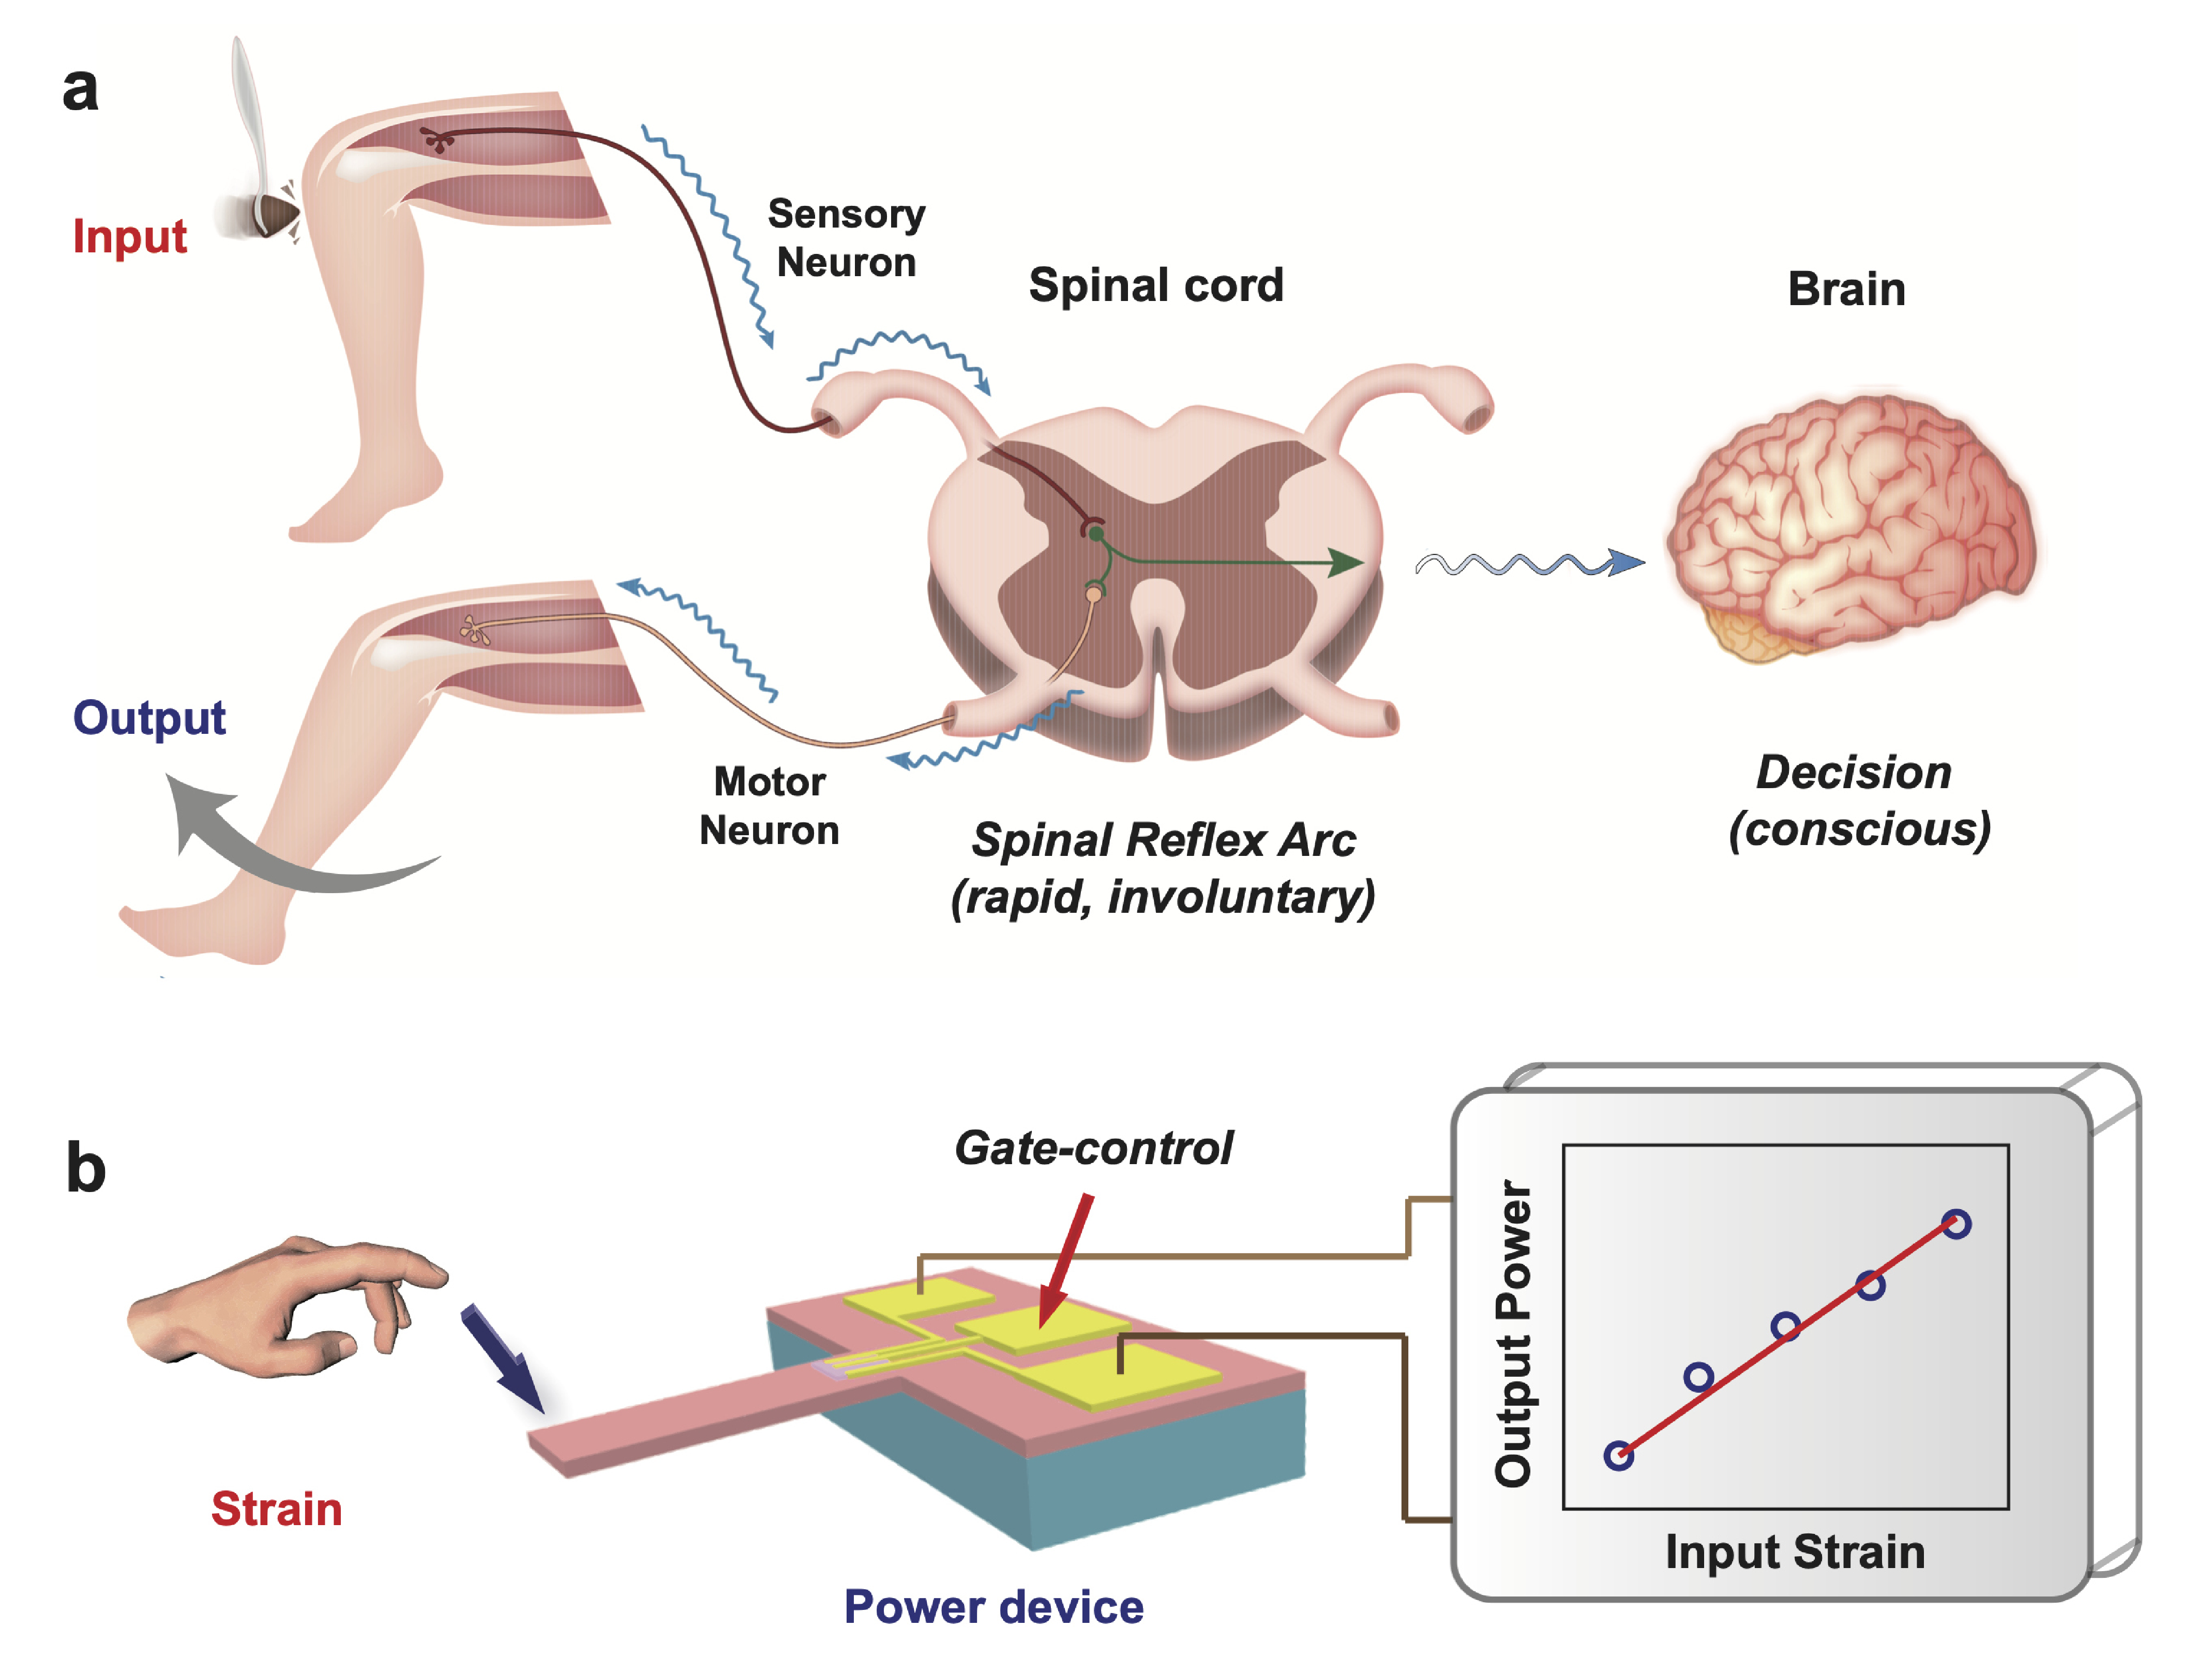
\includegraphics[width=0.9\textwidth]{ch3_concept}
\caption[Concept of strain-controlled power device (SPD) as inspired by human reflex]{Concept of strain-controlled power device (SPD) as inspired by human reflex}
\label{fig3:concept}
\end{figure}

\section{Design and preparation}
\label{sec:Design and preparation chapter2}

\subsection{Device structure and characterization}
\label{sec:Device structure and characterization chapter2}

The SPD \index{Strain-controlled power MEMS devices (SPD)} is designed by using the AlGaN/AlN/GaN heterojunction \index{AlGaN/AlN/GaN heterojunction} in a cantilever \index{Cantilever} architecture, as schematically shown in \autoref{tab:3.1} and \autoref{fig3:structure}a. The enlarged part is the schematic cross-section of the AlGaN/AlN/GaN heterostructure. The thicknesses of AlGaN, AlN, and GaN layers are 30 \unit{nm}, 1 \unit{nm} and 4.3 \unit{um}, respectively. The detailed fabrication process \index{Fabrication process} is described in the \autoref{sec:Fabrication processes chapter3}. The cantilever-based \index{Cantilever} structure of the as-fabricated SPD \index{Strain-controlled power MEMS devices (SPD)} is clearly shown in the scanning electron microscopy (SEM) \index{Scanning electron microscopy (SEM)} images of \autoref{fig3:structure}b. And the inset illustrates the geometry of gate and source-drain contacts. 

\begin{table}[H]
\renewcommand\arraystretch{1.5}
\centering
\caption[Structure parameters of the HEMT and SPD]{Structure parameters of the HEMT and SPD}
\begin{tabular}{ccccc}
\hline \hline
SPD design  & Material      & Length (\unit{um}) & Width (\unit{um})& Thickness (\unit{nm}) \\ \hline \hline
Cantilever  & GaN           & 350    & 50    & 5000      \\
HEMT & AlGaN/AlN/GaN & 27     & 27    & 30/1/4300 \\ \hline \hline
\end{tabular}
\label{tab:3.1}
\end{table}

\begin{figure}[H] 
\centering    
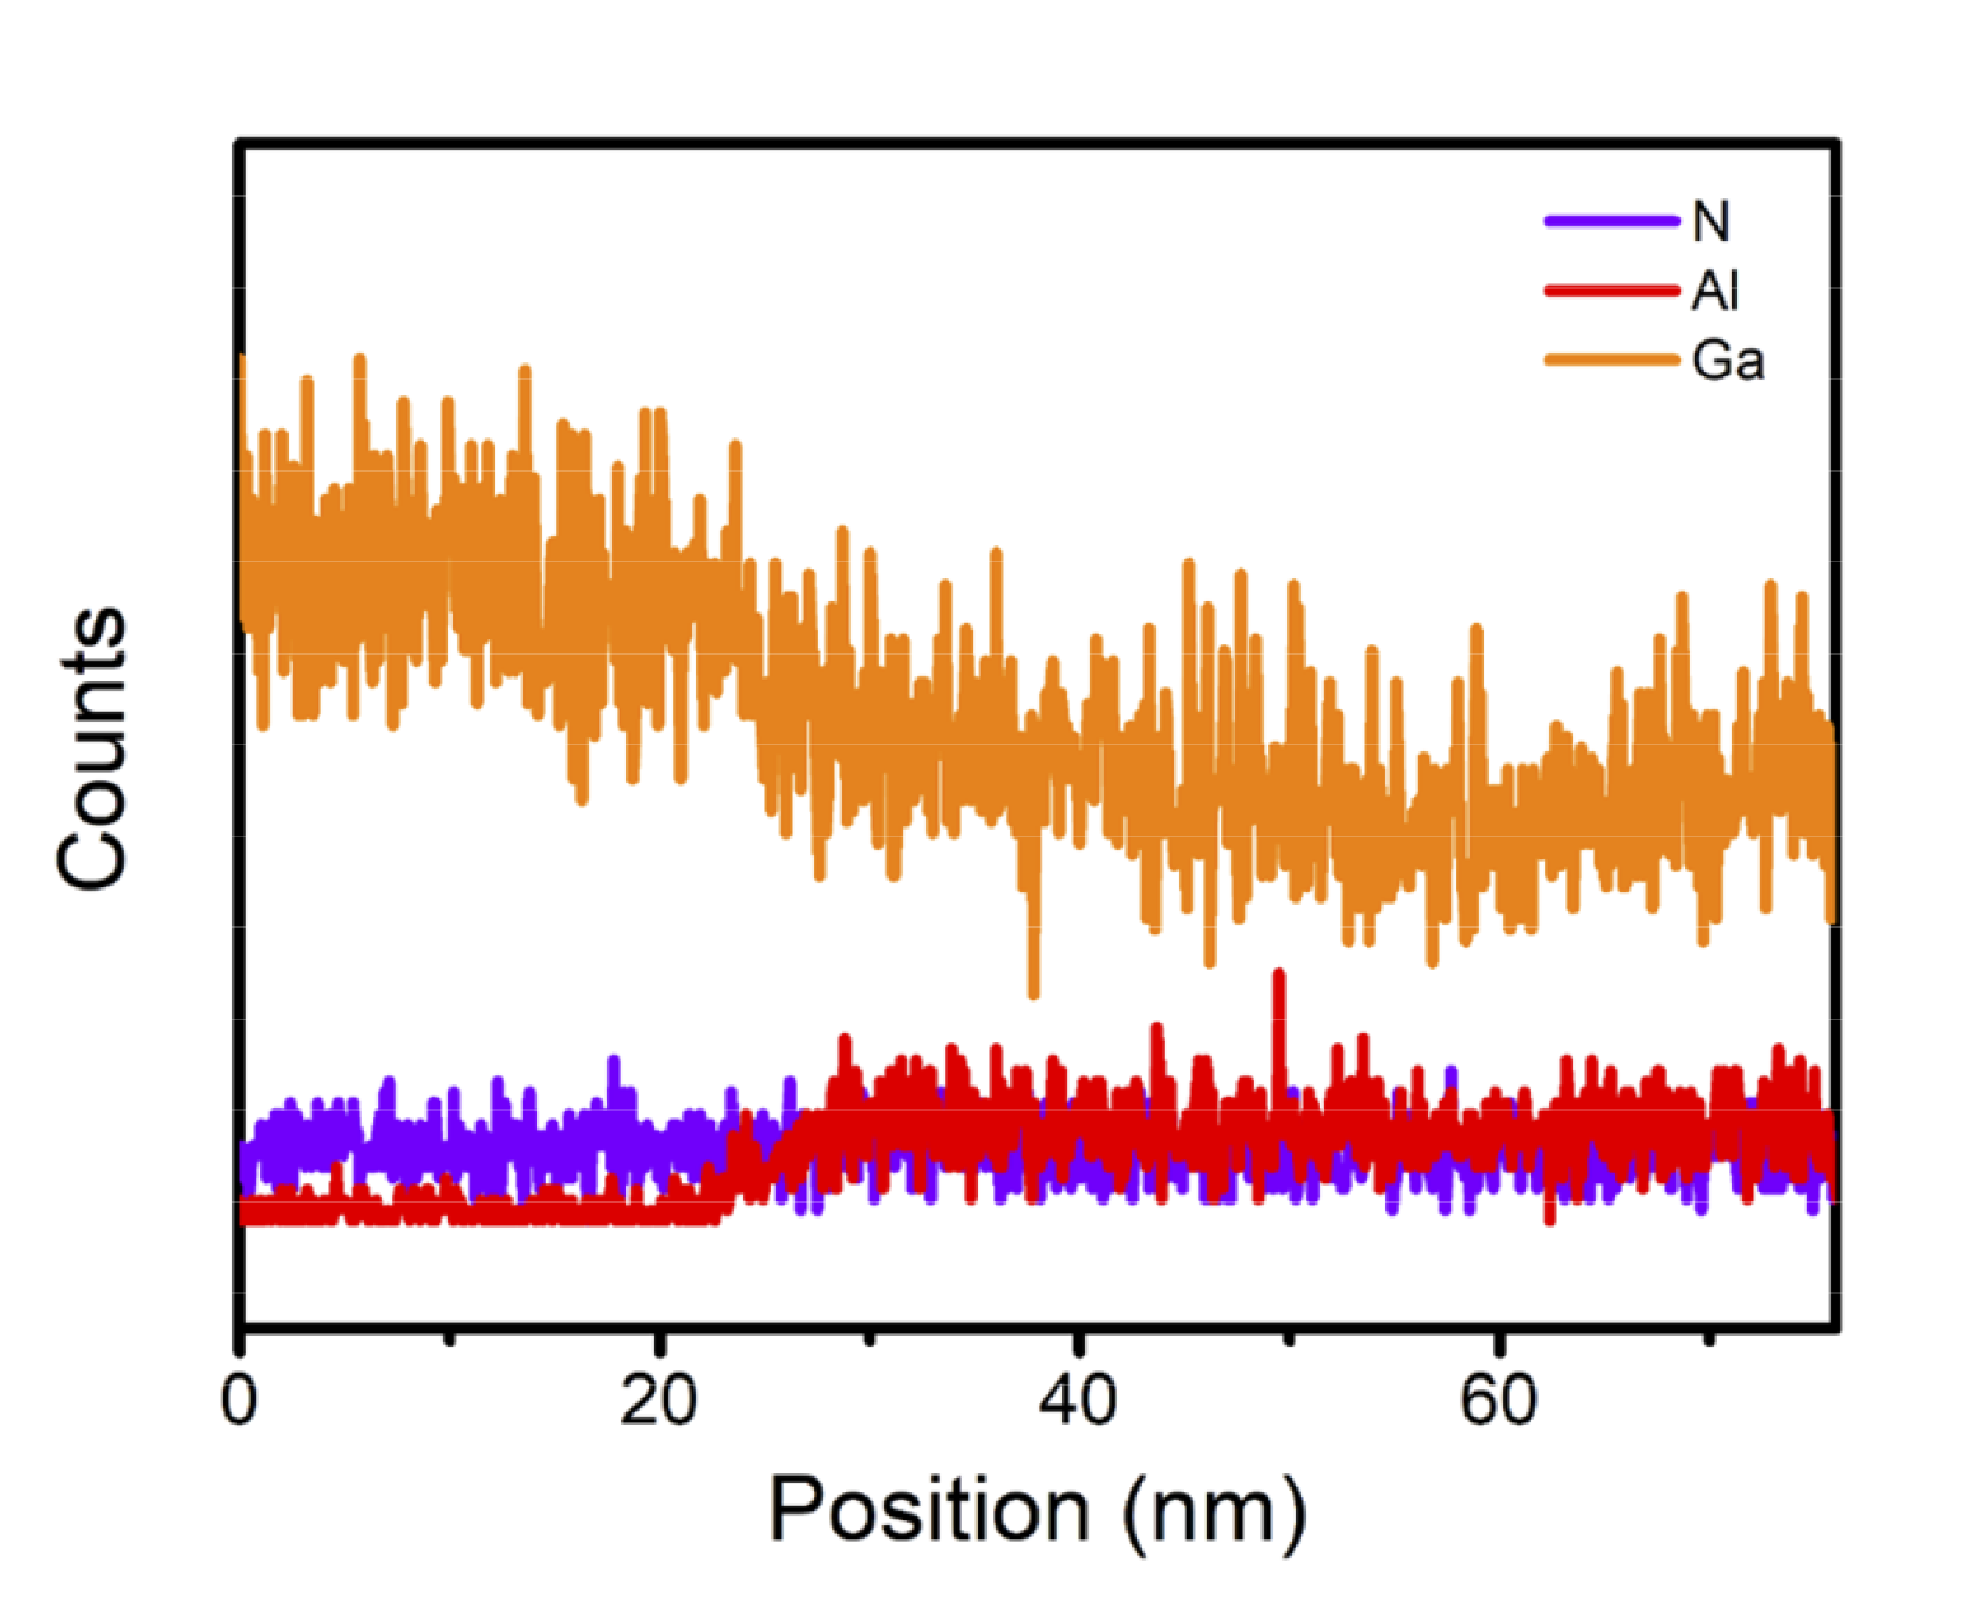
\includegraphics[width=0.6\textwidth]{ch3_edx}
\caption[EDX line profiles for the element of Ga (orange), Al (red), and N (purple)]{EDX line profiles for the element of Ga (orange), Al (red), and N (purple)}
\label{fig3:edx}
\end{figure}

The high-angle annular dark-field scanning transmission electron microscopy (HAADF-STEM) \index{Transmission electron microscopy (TEM)} images (\autoref{fig3:structure}c) exhibit the AlGaN/AlN/GaN heterostructure. Furthermore, the energy-dispersive X-ray spectroscopy (EDX) \index{Energy-dispersive X-ray spectroscopy (EDX)} elemental mapping (\autoref{fig3:structure}c) confirms the existence and corresponding distributions of the elements of Ga, Al, and N. The detailed structural information of the AlGaN/AlN/GaN heterostructure \index{AlGaN/AlN/GaN heterojunction} is investiated by high-resolution transmission electron microscopy (HRTEM) and selected area electron diffraction (SEAD) (inset of \autoref{fig3:structure}d). The interfaces atoms of AlGaN/AlN and AlN/GaN are uniform and sharp without apparent boundary defects or dislocations. The layers of GaN, AlN, and AlGaN can be easily identified, corresponding to the (0002) plane. Additionally, the corresponding line profile extracted from EDX mapping is presented in \autoref{fig3:edx}, confirming the variation of chemical compositions.


\begin{figure}[H] 
\centering    
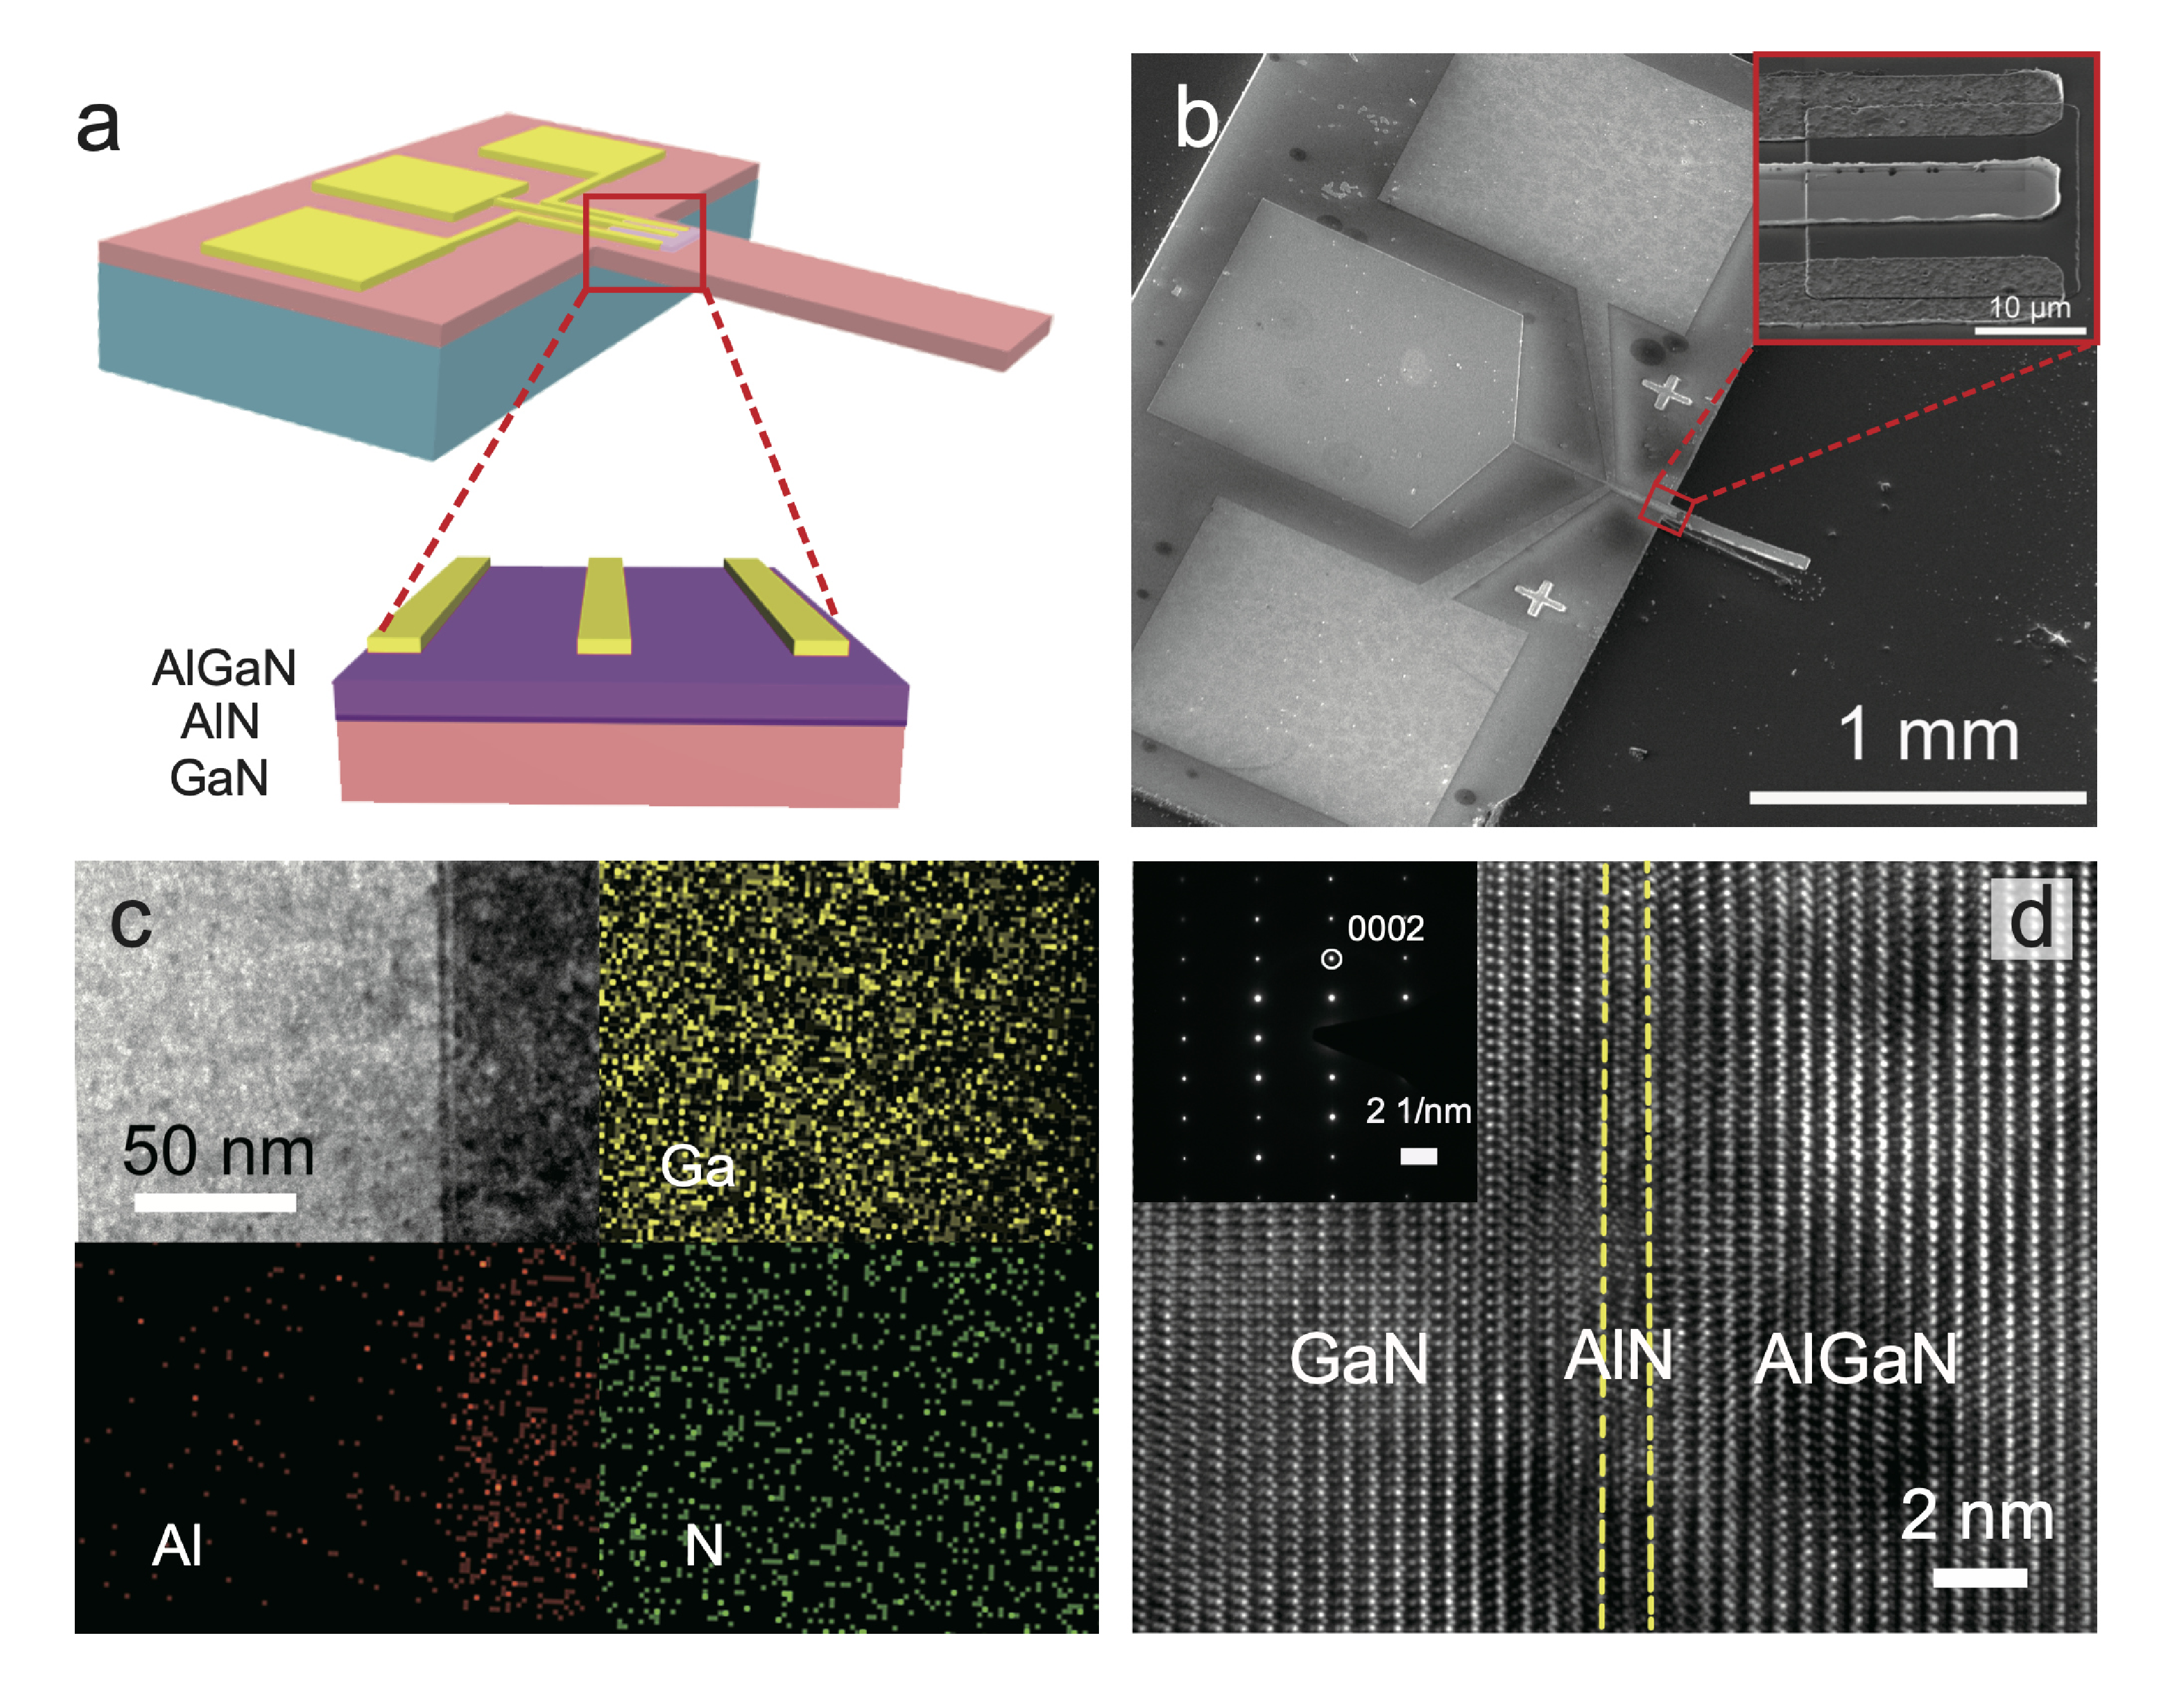
\includegraphics[width=0.9\textwidth]{ch3_structure}
\caption[Structure and material characterizations of the SPD]{Structure and material characterizations of the \index{Strain-controlled power MEMS devices (SPD)} SPD. (a) Schematic illustration and (b) SEM image of the SPD. (c) Cross-sectional HAADF-STEM image and the EDX element mapping, as well as the (d) TEM image of the AlGaN/AlN/GaN hetero-stacks.}
\label{fig3:structure}
\end{figure}


\subsection{Fabrication processes}
\label{sec:Fabrication processes chapter3}

We develop a fully dry etching \index{Etching!dry etching} process by using the inductively coupled plasma etching (ICP) \index{Inductively coupled plasma (ICP)} to fabricate the GaN-based \index{Cantilever} cantilever, and the details of the ICP-based dry etching steps are schematically shown in \autoref{fig3:etch}. The two key procedures are illustrated as follows: (i) trenches are fabricated by anisotropic etching \index{Etching!anisotropic etching} of GaN/Si (\autoref{fig3:etch}b). The photoresist \index{Photoresist} patterned GaN \index{Thin film} thin film (thickness: 5 \unit{\um}) was completed etched by using the anisotropic etching recipe (\ce{BCl3}/\ce{Cl2}/\ce{Ar}: 10/32/5 sccm; Power: \SI{550}{\watt}; Process time: 20 \unit{\minute}); (ii) the cantilever \index{Cantilever} structure is laterally released by isotropic etching of Si (\autoref{fig3:etch}c). The cantilever \index{Cantilever} structure was fabricated with the isotropic etching recipe (\ce{SF6}/\ce{O2}/\ce{Ar}: 30/5/10 sccm; Power: \SI{800}{\watt}; Process time: 25 \unit{\minute}). The manufactured cantilever \index{Cantilever} had dimensions of \numproduct{350 x 50 x 5 } \unit{\cubic\um}, with the embedded HEMT had a mesa dimension of \numproduct{27 x 27} \unit{\square\um} and a gate length of 5 \unit{\um}. The anisotropic / isotropic etching \index{Etching!isotropic etching} steps can be easily controlled by simply adjusting the etching recipe (e.g., gas mixture, power, and time). The presented fully dry etching process has many unique advantages including precise control, well-aligned shape, less-contaminated, and easily-integrated into Si-based circuits.

\begin{figure}[H] 
\centering    
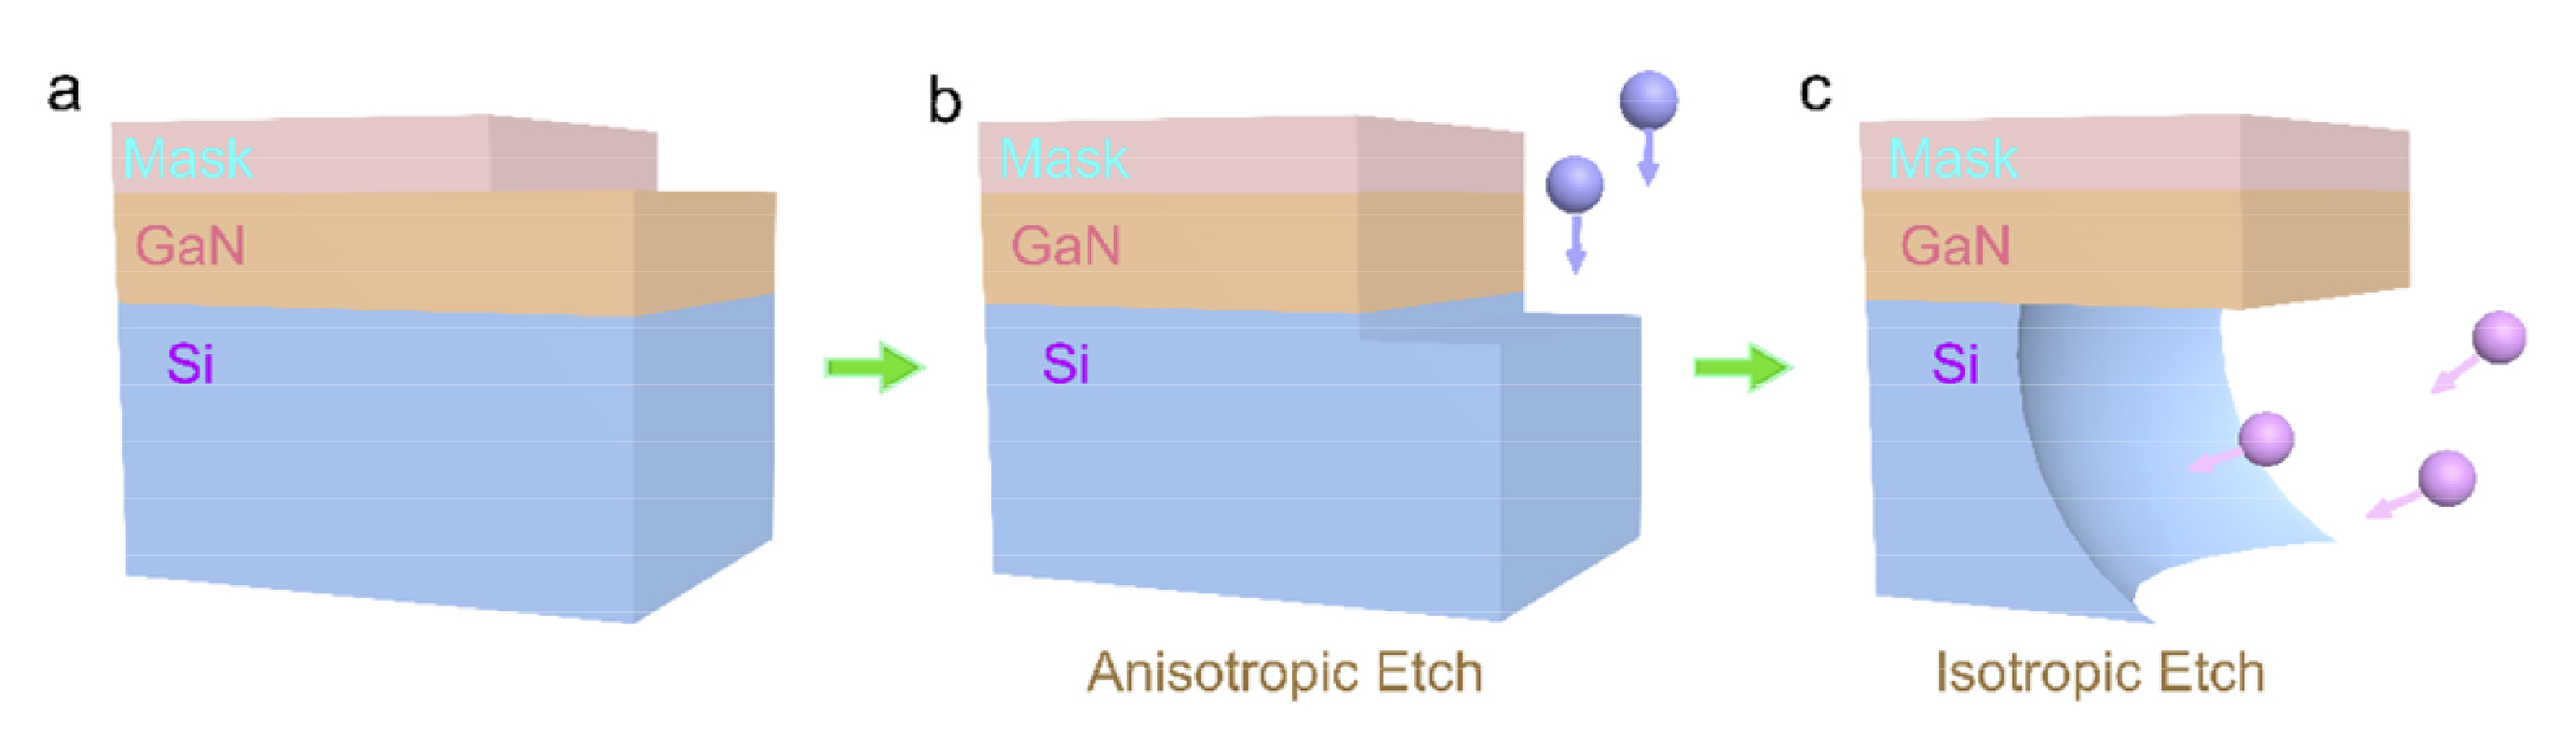
\includegraphics[width=0.9\textwidth]{ch3_etch}
\caption[Etching process flow chart of the SPD]{Etching process flow chart of the SPD. (a) Patterning the cantilever with positive photo resist. (b) Fabricating a trench by anisotropic etching of GaN/Si. (c) Releasing the cantilever structure by isotropic etching of Si.}
\label{fig3:etch}
\end{figure}

The SPD \index{Strain-controlled power MEMS devices (SPD)} was fabricated using III-Nitride \index{Nitride} epitaxial layers \index{Epitaxial!layer} by metal-organic chemical vapor deposition (MOCVD) \index{MOCVD} on Si substrate \index{Substrate} (111) with the 2DEG \index{Two-dimensional electron gas (2DEG)} sheet density of \num{8e12} $\sim$ \num{1e13} \unit{\per\square\cm}. The epitaxial layer structure consists of AlGaN (30 \unit{nm}, 30$\%$ Al) / AlN (1 \unit{nm}) / GaN (4.3 \unit{um}) / AlGaN buffer layer / Si substrate. The mesa and cantilever \index{Cantilever} patterns were etched using an inductively coupled plasma etching system (ICP, SENTECH SI 500) \index{Inductively coupled plasma (ICP)} etch process based on \ce{BCl3}/\ce{Cl2}/\ce{Ar} and \ce{SF6}/\ce{O2}/\ce{Ar}. Ti/Al/Ni/Au (20 \unit{nm} / 120 \unit{nm} / 45 \unit{nm} / 55 \unit{nm}) metal stack deposition was evaporated using electron beam evaporation \index{Deposition!electron beam evaporation} system (Denton Vacuum Explore 14) and annealed at \SI{850}{\degreeCelsius} in \ce{N2} environment for 30 \unit{\s} to form an ohmic contact \index{Contact!Ohmic contact} using a rapid thermal processing \index{Rapid thermal!processing (RTP)} system (LABSYS RTP-1200). Ni/Au (80 \unit{nm} / 50 \unit{nm}) was evaporated for gate metallization to form Schottky \index{Contact!Schottky contact} contacts. Finally, the ICP-based dry etching was performed by combing the anisotropic/isotropic etching to release the \index{Cantilever} cantilever, as schematically illustrated in \autoref{fig3:etch}.  The fabrication process \index{Fabrication process} flow is detailed in \autoref{fig3:process}.

\begin{figure}[H] 
\centering    

\includegraphics[width=0.9\textwidth]{ch3_process}
\caption[Fabrication process flow chart of the SPD]{Fabrication process flow chart of the SPD. (a) A diced chip with AlGaN/AlN/GaN epilayers grown on Si substrate. (b) The mesa etching of AlGaN, AlN and GaN by ICP. (c) Deposition of Ohmic contact and Schottky contact. (d) Cantilever preparation by ICP etching.}
\label{fig3:process}
\end{figure}


\section{Device performance}
\label{sec:Device performance chapter3}

\subsection{Electrical performance}
\label{sec:Electrical modulation chapter3}

 The measured \index{Contact!Schottky contact} contact \index{Contact!Ohmic contact} characteristics of the source-drain contact and gate contact of the SPD \index{Strain-controlled power MEMS devices (SPD)} and the HEMT are shown in \autoref{fig3:spdcontact}a, b and \autoref{fig3:hemt}a, b, respectively. Both the SPD and the HEMT exhibit typical Ohmic and Schottky contacts. Based on the suitable contacts, the output characteristics ($I_{ds}$-$V_{ds}$) of the SPD \index{Strain-controlled power MEMS devices (SPD)} and the\index{HEMT} HEMT show good capability of gate-control, as respectively shown in \autoref{fig3:performance}a and \autoref{fig3:hemt}c. The output characteristics show a distinct linear region at a low source-drain bias ($V_{ds}$), and then the drain current \index{Current!drain current} approaches saturation with further increasing of the drain bias. Large output currents \index{Output!current} are achieved in both SPD and HEMT and can be effectively controlled at various $V_{gs}$ of \SI{-5}{\volt} to \SI{1}{\volt}. When compared to the HEMT, the SPD shows a reduced current of 60 \unit{\mA\per\mm} at \SI{10}{\volt} because of its suffering from strain \index{Strain} partial release and more dry etching \index{Etching!dry etching} process. Furthermore, the transfer ($I_{ds}$–$V_{gs}$) characteristics of the SPD \index{Strain-controlled power MEMS devices (SPD)} and the HEMT at $V_{ds}$ = \SI{6}{\volt} are shown in \autoref{fig3:performance}b and \autoref{fig3:hemt}d, respectively. The maximum transconductance \index{Transconductance} ($g_{m,max}$) of 7.5 \unit{\milli\siemens\per\mm} is measured in the SPD (\autoref{fig3:performance}b), while the value for the HEMT can reach 52 \unit{\milli\siemens\per\mm} (\autoref{fig3:hemt}d). 

\begin{figure}[H] 
\centering    
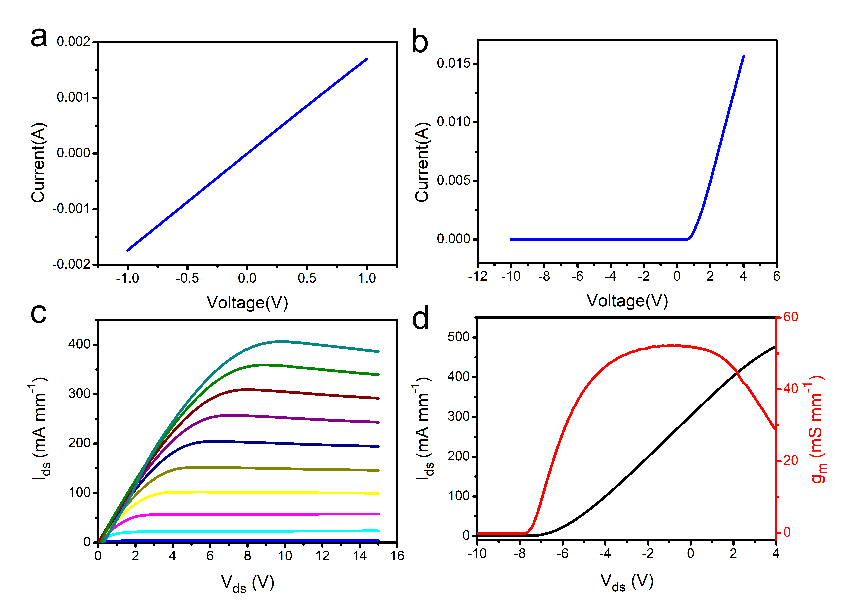
\includegraphics[width=0.9\textwidth]{ch3_hemt}
\caption[Electrical performance of the HEMT]{Electrical performance of the HEMT. (a) Ohmic contact characteristics. (b) Schottky contact characteristics. (c) Output characteristics. (d) Transfer characteristics}
\label{fig3:hemt}
\end{figure}


\begin{figure}[H] 
\centering    
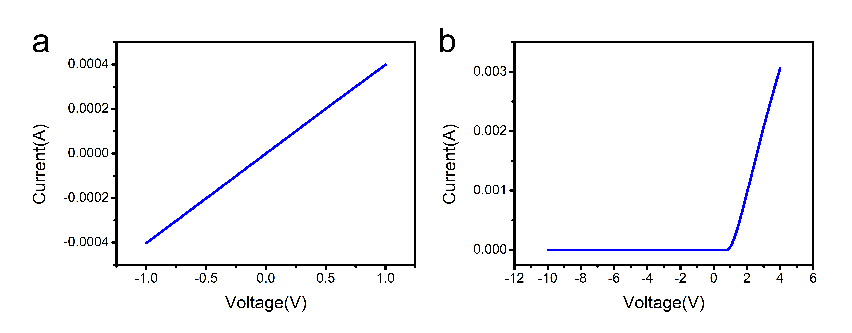
\includegraphics[width=0.9\textwidth]{ch3_spdcontact}
\caption[Contact characterizations of the SPD]{Contact characterizations of the SPD (a) Ohmic contact curve. (b) Schottky contact curves.}
\label{fig3:spdcontact}
\end{figure}

To further investigate the reason for the degradation \index{Degradation} of SPD performance before and after etching, we measured the micro-Raman spectra of SPD \index{Strain-controlled power MEMS devices (SPD)} and \index{HEMT} HEMT at room temperature (\autoref{fig3:performance}c). It can be seen that the $E_{2h}$ phonon mode peak of GaN in SPD shows a blue-shift of Raman phonon frequency \index{Raman!phonon frequency} from 566.8 to 569.2 \unit{\per\cm} compared to HEMT. It revealed that the ICP etching process during the fabrication of the \index{Cantilever} cantilever induces tensile strain relaxation of the GaN layer \cite{yang2015influence}, which is due to the lattice mismatch \index{Lattice!mismatch} between the III-V \index{Nitride} nitride and the silicon \index{Substrate} substrate. The lattice constant \index{Lattice!constant} of GaN typically is \SI{3.189}{\angstrom}, while Si has a lattice constant \index{Lattice!constant} of \SI{5.43}{\angstrom}, which results in severe tensile strain in the GaN layer \cite{cheng2015high}. Due to the strong piezoelectric effect \index{Piezoelectric!effect} of III-V nitrides, lattice strain \index{Lattice!strain} can generate corresponding piezoelectric polarization charges \index{Piezoelectric!polarization charge} at the interface \index{Interface} of the GaN layer, thereby modulating the energy band \index{Energy band} structure of the AlGaN/AlN/GaN \index{AlGaN/AlN/GaN heterojunction} heterojunction, and ultimately affecting the carrier concentration \index{Carrier!concentration} and other electrical properties in heterojunctions. Therefore, when the Si substrate is removed by an isotropic etching \index{Etching!isotropic etching} process, the tensile strain of the GaN layer is partially released \cite{choi2013analysis}, which significantly weakens the piezoelectric polarization charge density \index{Piezoelectric!polarization charge} and reduces the 2DEG concentration \index{Two-dimensional electron gas (2DEG)} in AlGaN/AlN/GaN interface \cite{ambacher1999two}. On the other hand, since the ICP etching time is as long as $45$ minutes in the cantilever \index{Cantilever} fabrication process, the long etching time will introduce a large number of defects in the SPD \index{Strain-controlled power MEMS devices (SPD)} lattice \index{Lattice!defects} \cite{ladroue2010deep,pearton2000review,huang2004inductively,lan2006icp,fang2003etching}, thus reducing the electrode \index{Electrode} contact performance in the SPD \index{Strain-controlled power MEMS devices (SPD)} active \index{Active region} area. It will also degrade the final electrical performance to some extent. Therefore, how to protect the SPD during the long-time etching process is the key to improve the device performance. In the process of MPD device preparation in \autoref{ch:Magnetosensory Power Devices}, we propose a method of applying multi-layer photoresist to further protect the active area \index{Active region} of MPD device during the etching process, and the experimental results show that the device performance of MPD has been significantly improved. The relevant discussion will be expanded \index{Current!drain current} in \autoref{ch:Magnetosensory Power Devices}.

\begin{figure}[H] 
\centering    
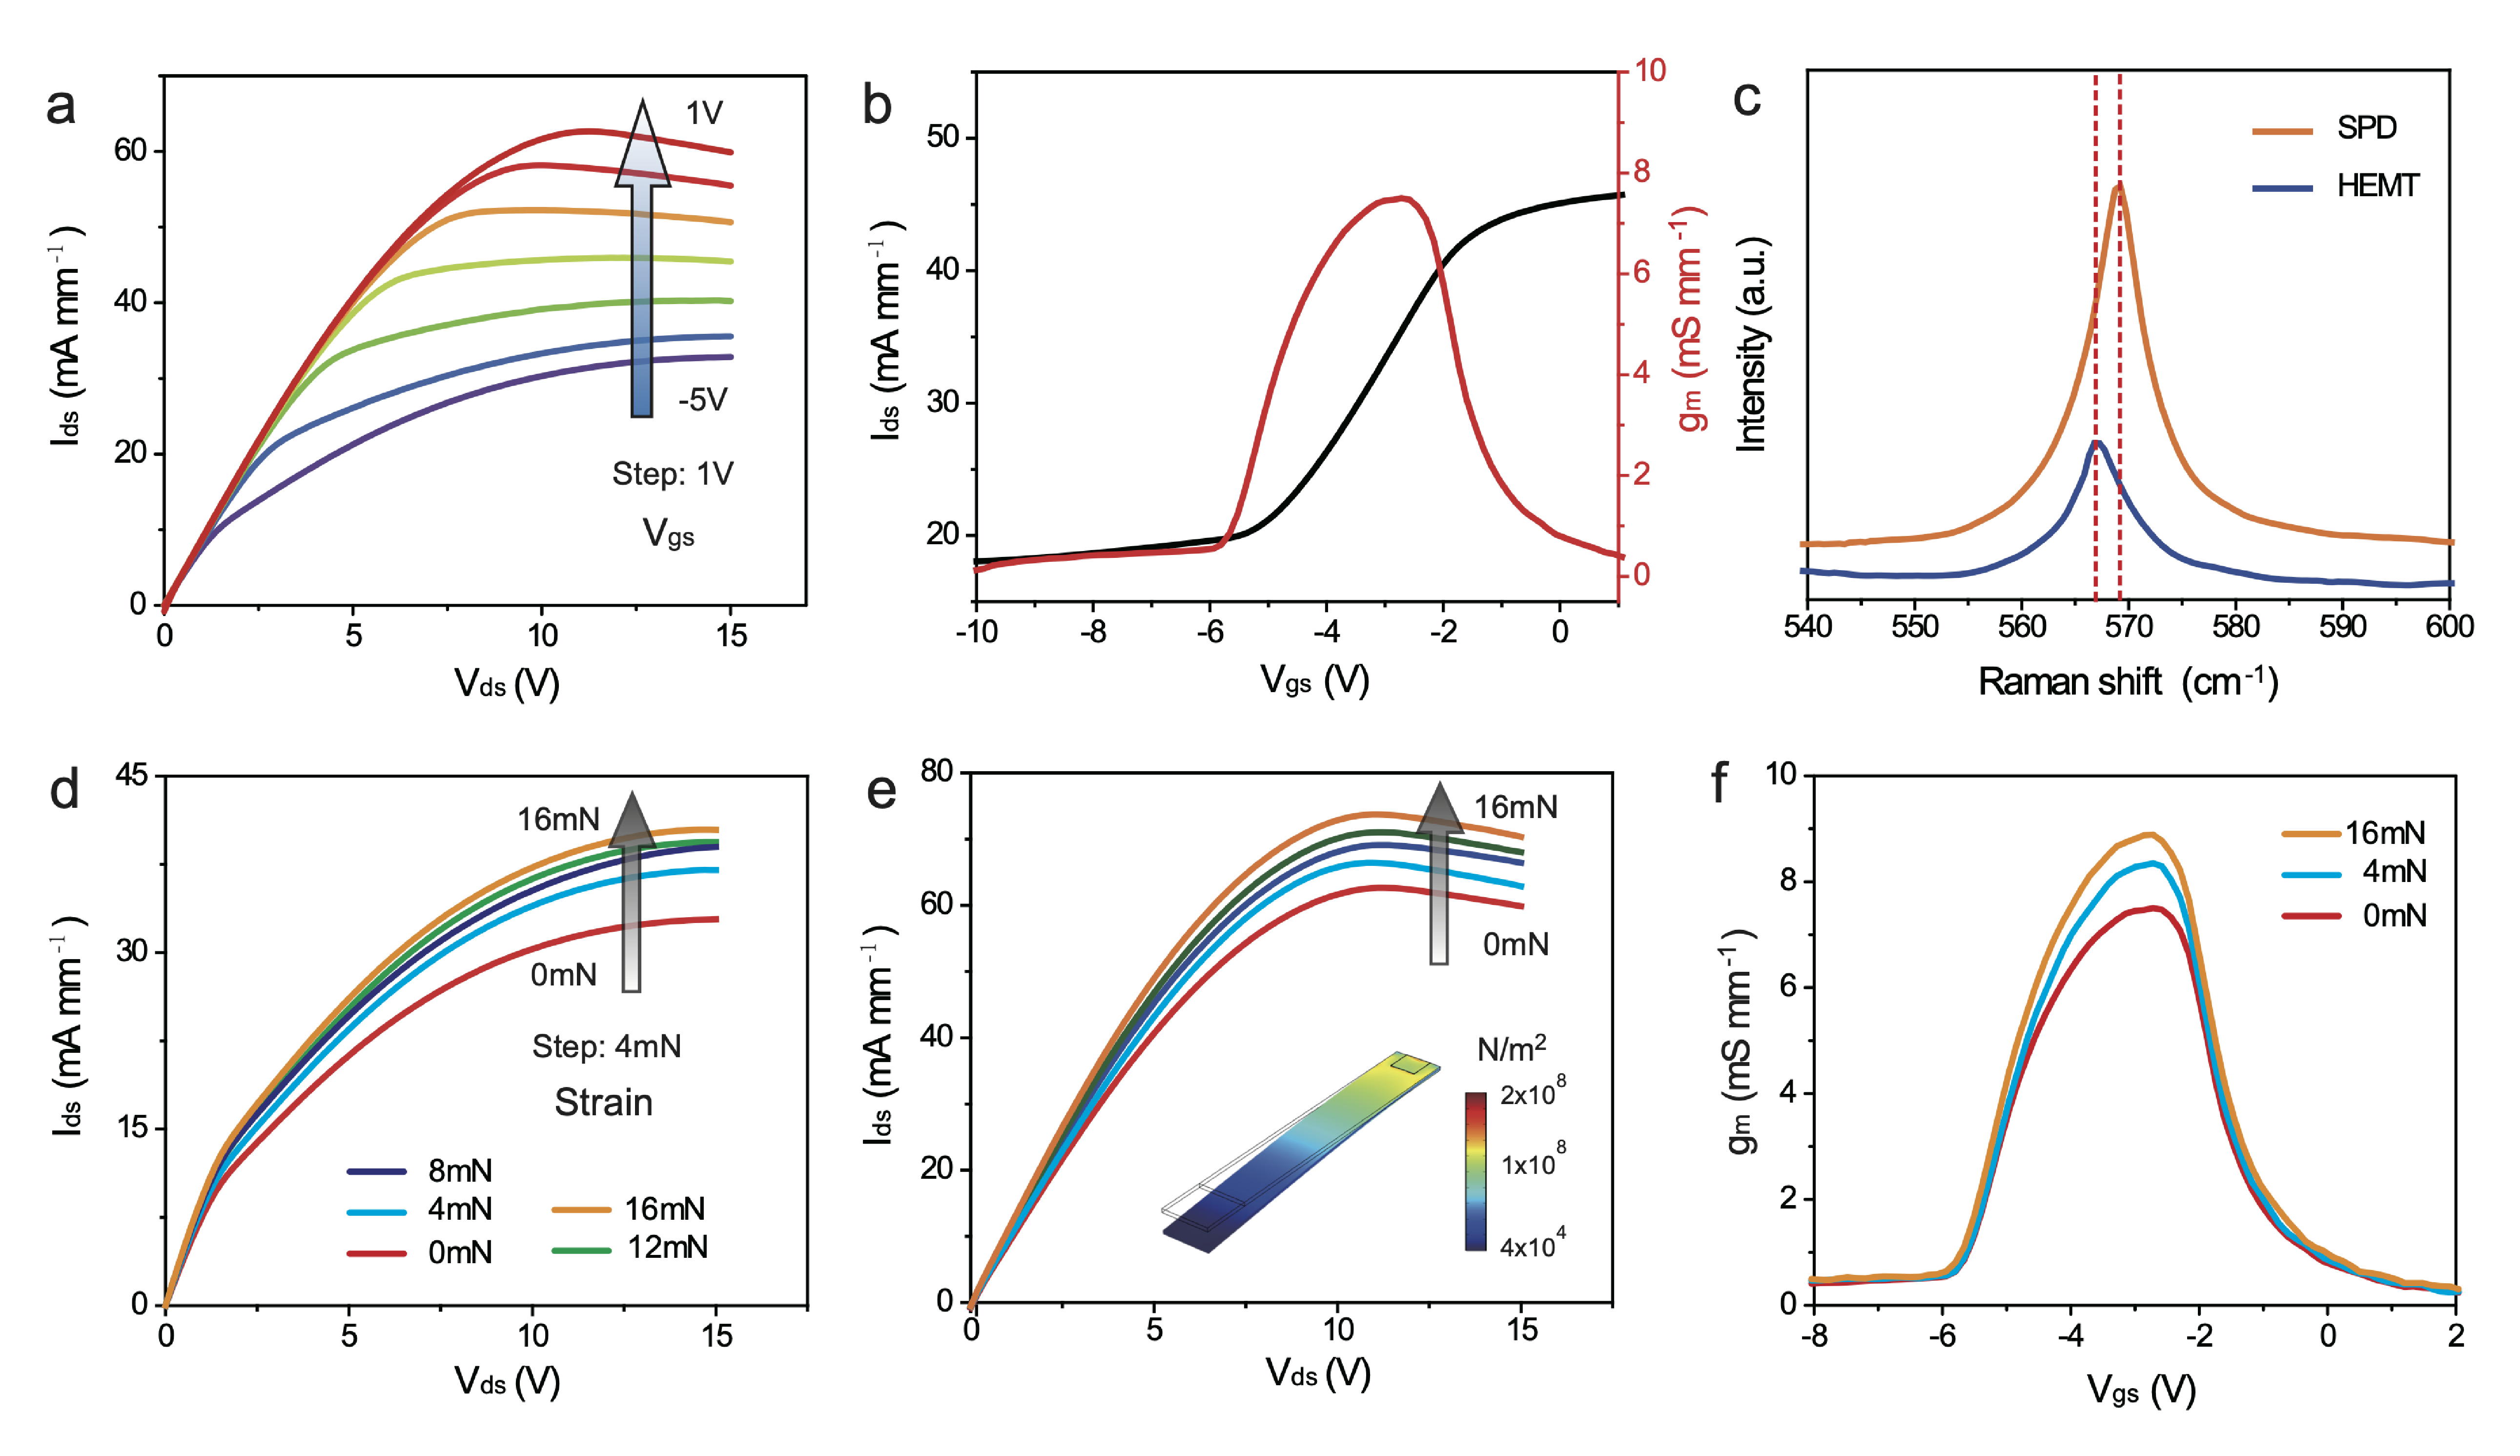
\includegraphics[width=0.9\textwidth]{ch3_performance}
\caption[Electrical performance of the SPD]{Electrical performance of the SPD. (a) Output characteristics. (b) Transfer characteristics. (c) Spatial Raman spectra of the AlGaN/AlN/GaN heterostructures before (HEMT) and after (SPD) dry-etching. (d), (e) Output characteristics under external strain from 0 $\sim$ 16 \unit{\mN}, with the gate voltage $V_{gs}$ of (d) \SI{-5}{\volt} and (e) \SI{1}{\volt}, respectively. The inset of (e) illustrates the strain distribution of the SPD under an external strain of 16 \unit{\mN}. (f) The transconductance under various external strain.}
\label{fig3:performance}
\end{figure}

\subsection{Strain-power modulation performance}
\label{sec:Strain-power modulation}

Based \index{Finite element analysis} on \index{Cantilever} the piezotronics \index{Piezotronics} effect, the \index{Current!drain current} output power of the \index{Strain-controlled power MEMS devices (SPD)} SPD can be effectively modulated by external mechanical stimulus in real time. The external strain is loaded on the free-end of the

\begin{figure}[H] 
\centering    
\includegraphics[width=0.8\textwidth]{ch3_modulation3}
\caption[Strain-controlled output power characteristics at various gate voltage]{Strain-controlled \index{Current!drain current} output power characteristics at various gate \index{Strain-controlled power MEMS devices (SPD)} voltage}
\label{fig3:modulation3}
\end{figure}

\noindent cantilever by using a probe needle loaded along the c-axis direction. An increase in in-plane tensile strain occurs in the AlGaN/AlN/GaN heterostructure. The deflection depth of the cantilever can be tuned by the probe needle in the controllable/reproducible manners. And the loaded strain can be calculated with material mechanics equations. And thus, the normal force increases from 0 to 16 \unit{\mN} as the deflection depth of the cantilever increases from 0 to 20 \unit{\um}.

In order \index{Current!drain current} to further understand the strain effect on the output characteristics of the \index{Strain-controlled power MEMS devices (SPD)} SPD, different external strains are loaded on the free-end of the cantilever. It can be clearly observed that the $I_{ds}$–$V_{ds}$ curves show up-shifts to some degrees according to the increasing of the strain, which are both shown in \autoref{fig3:performance}d, e. It means a direct and effective output power \index{Output!power} modulation by a weak mechanical stimulus. As applying an external strain along c-axis, a piezo-potential is generated, resulting in the change of 2DEG \index{Two-dimensional electron gas (2DEG)} and thus modulating electron transport. It should be noted that the SPD is a high-power device capable of directly controlling electricity rather than a strain sensor.

In addition, the output current \index{Output!current} response to the external strain is also effectively modulated by the $V_{gs}$. The controllable capabilities of various $V_{gs}$ (\SI{-5}{\volt} $\sim$ \SI{1}{\volt}) under strains of 0 $\sim$ 16 \unit{\mN} are presented in \autoref{fig3:performance}d, e and \autoref{fig3:modulation3}a–e, respectively. It can be clearly seen that a progressively higher modulation of current density is directly controlled at a $V_{gs}$ of \SI{1}{\volt} with the same strain. When the cantilever \index{Cantilever} is subjected to an external strain, the output current density of the cantilever increases, both in the linear region or the saturation region. The saturated current at $V_{ds}$ = \SI{15}{\volt} reaches 40.43 \unit{\mA\per\mm} under the maximum applied pressure (or strain of 16\unit{\mN}) compared to the SPD without strain (32.83 \unit{\mA\per\mm} at $V_{gs}$ = \SI{-5}{\volt}. In contrast, the output current can be reached 70.36 \unit{\mA\per\mm} compared to the SPD without strain (59.87 \unit{\mA\per\mm}) at $V_{gs}$ = \SI{1}{\volt}. It indicates that the SPD sensitivity is programmable. The inset of \autoref{fig3:performance}e illustrates the strain distribution of the SPD under an external strain of 16 \unit{\mN}, which is simulated by COMSOL Multiphysics. Besides, the transconductance of the SPD \index{Strain-controlled power MEMS devices (SPD)} at different applied external strain is displayed in \autoref{fig3:performance}f. The transconductance shows an in-


\begin{figure}[H] 
\centering    
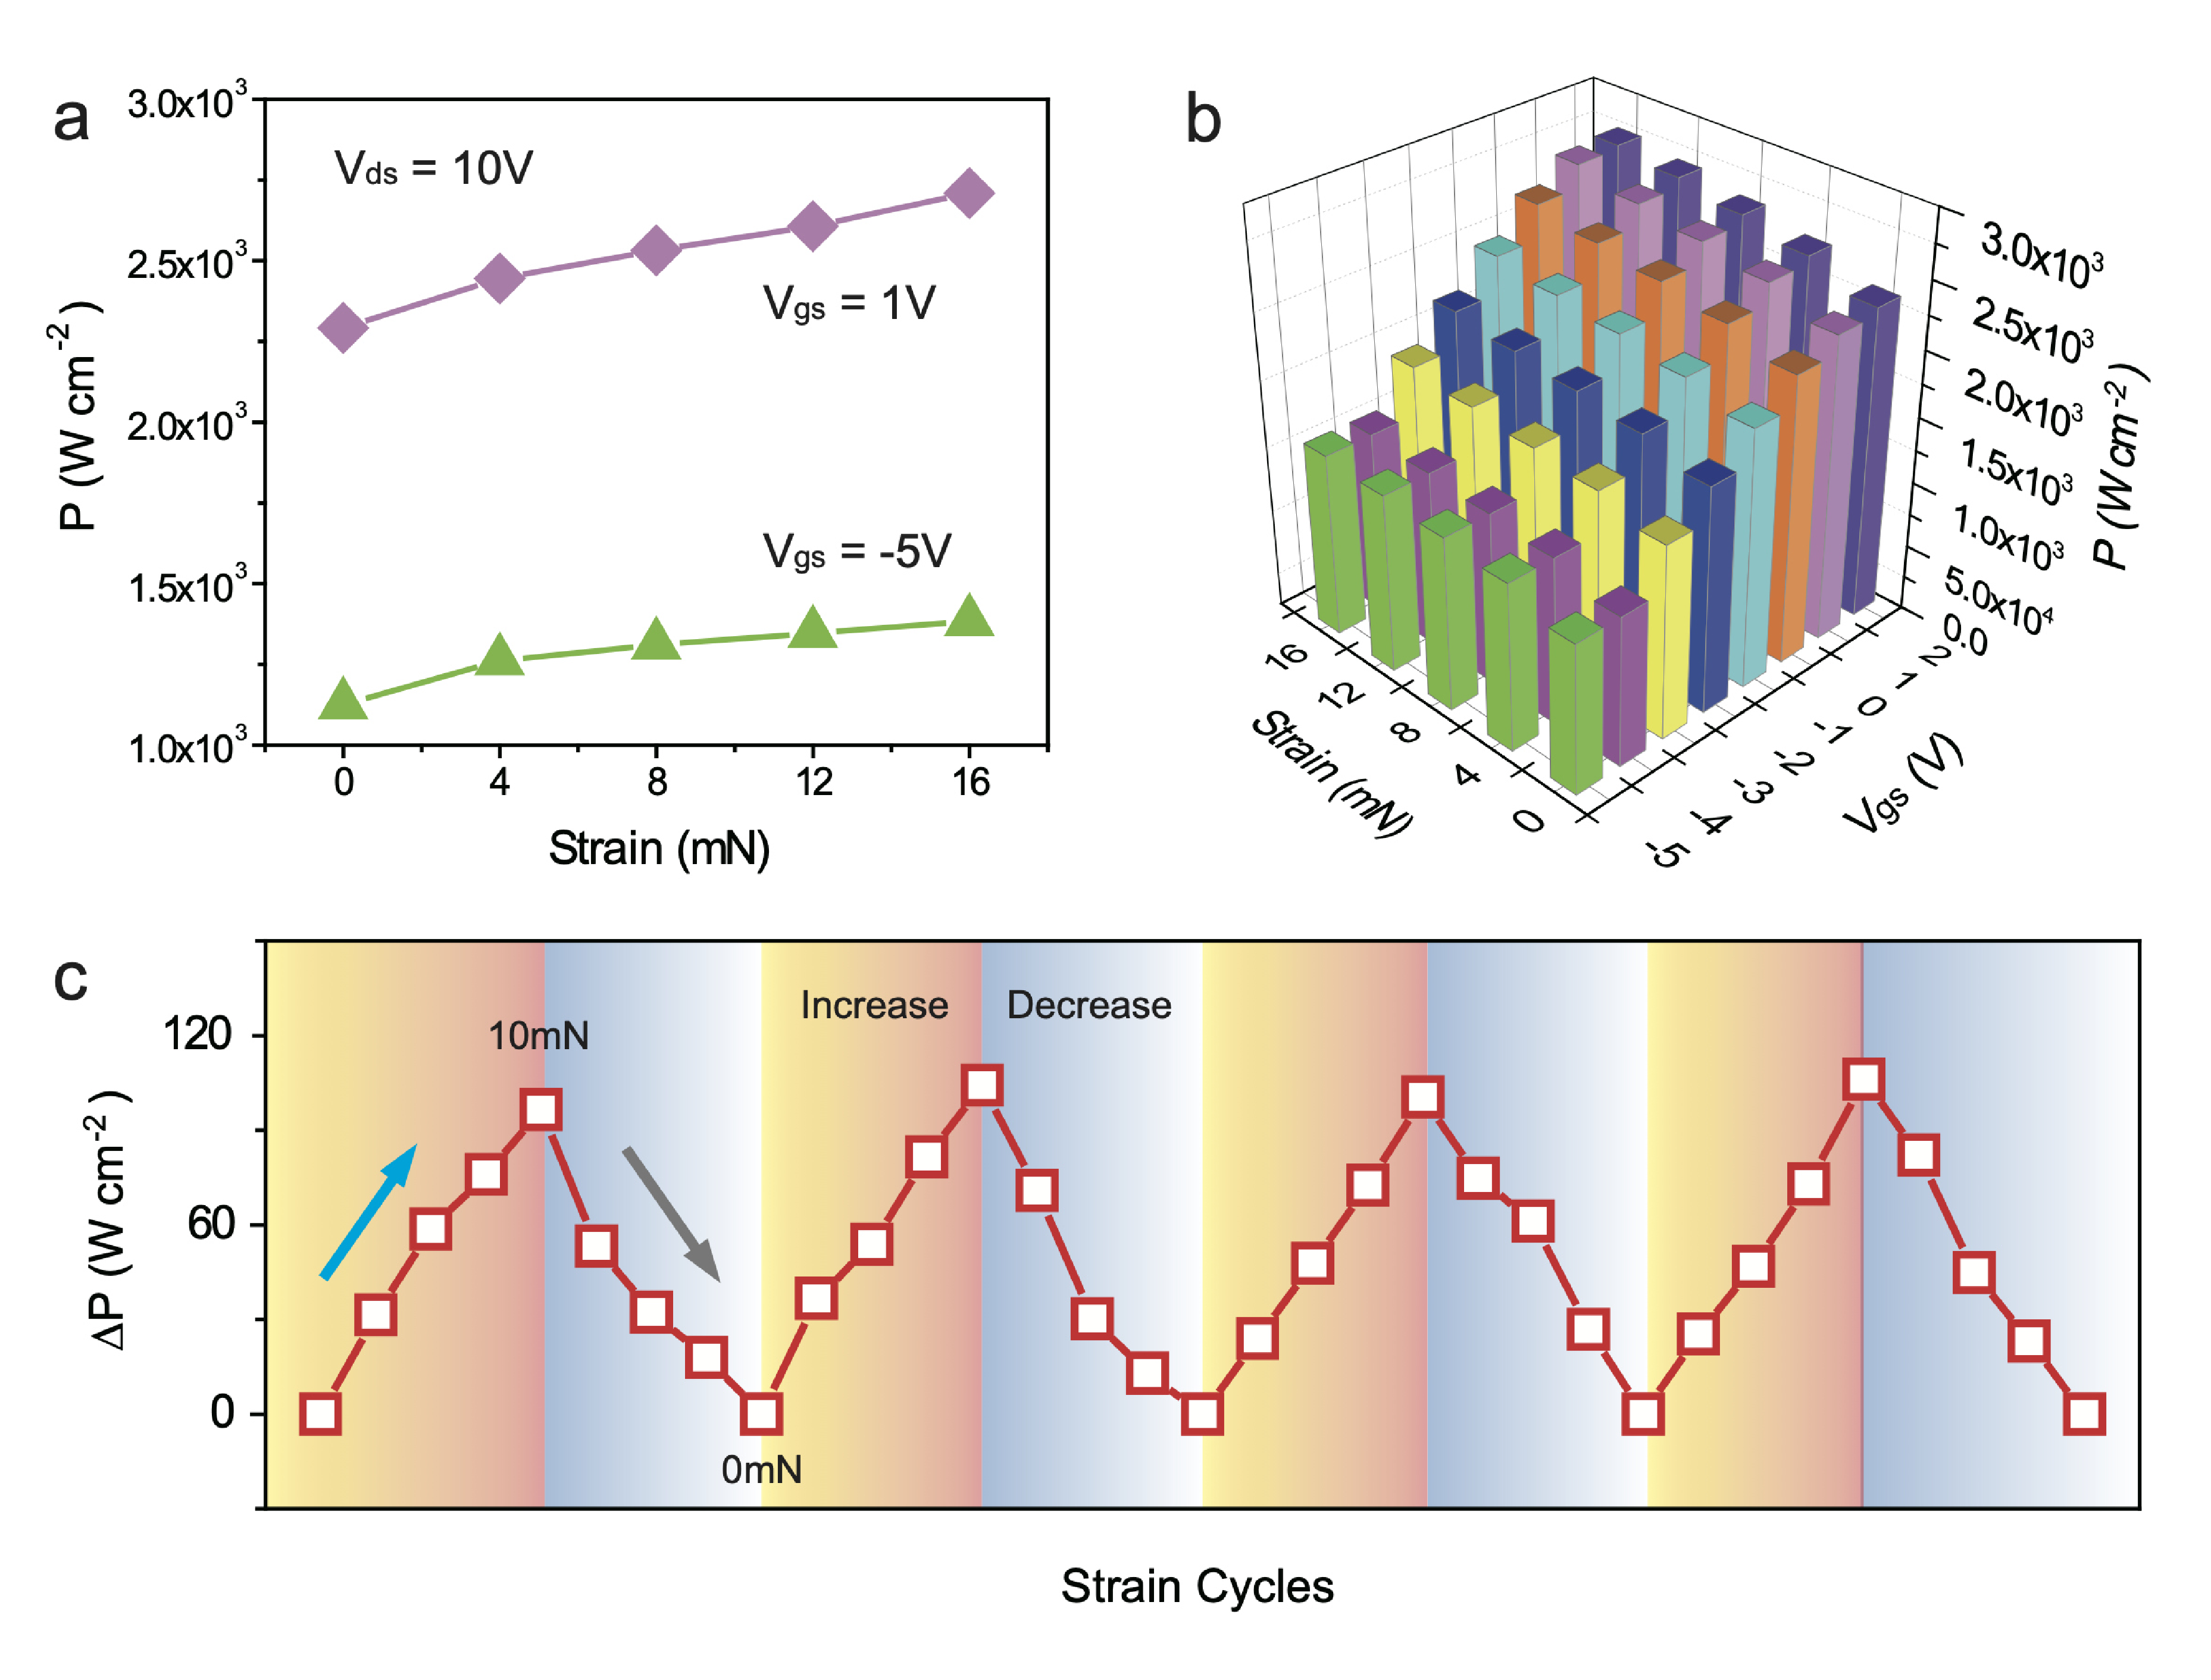
\includegraphics[width=0.9\textwidth]{ch3_modulation1}
\caption[Strain-controlled output power characteristics of SPD]{Strain-controlled output power characteristics of SPD. (a) Output power density under external strain from 0 to 16 \unit{\mN} at $V_{gs}$=\SI{-5}{\volt} and $V_{gs}$=\SI{1}{\volt}. (b) 3D plots illustrating the relationship between the output power density and the input strain or gate voltage. (c) Reproducible procedures of loading or unloading strain (0 $\sim$ 10 \unit{\mN}) in response to the relative output power density in cyclic tests.}
\label{fig3:modulation1}
\end{figure}

\noindent -crease with the increasing of applied external strain, indicating that the gate has an increasingly stronger capability to control the channel \index{Channel} current. Therefore, it proves that the piezotronics \index{Piezotronics} effect, i.e., strain-controlled behavior, can effectively modulate the output characteristics of the SPD.

The output power \index{Output!power} modulation \index{Modulation} of the SPD \index{Strain-controlled power MEMS devices (SPD)} is further discussed. \autoref{fig3:modulation1}a shows the relationship between output power density and different strain. The output power density dependence on the applied strain can be obtained by employing strain-controlled output characteristics. More specifically, the output power density shows an increase with the applied strain (0 $\sim$ 16 \unit{\mN}), as a result of the increasing of the additional electrons and concentrations of 2DEG \index{Two-dimensional electron gas (2DEG)} suffering from in-plane tensile strain. The maximum output power density of the SPD \index{Strain-controlled power MEMS devices (SPD)} can reach \num{1.39e3} \unit{\W\per\square\cm} and \num{2.72e3} \unit{\W\per\square\cm}, respectively, in response to the $V_{gs}$ of \SI{-5}{\volt} and \SI{1}{\volt} under the strain of 16 \unit{\mN}. Furthermore, the output power level can also be tuned at the different $V_{gs}$, as shown in \autoref{fig3:modulation1}a, b, and \autoref{fig3:modulation3}f–j. Upon the strain of 16 \unit{\mN}, the relative output power density increases up to 1.51, 1.74, 2.02, 2.29, and \num{2.54e3} \unit{\W\per\square\cm}, respectively, at different $V_{gs}$ (\autoref{fig3:modulation3}f–j). To check the sensitivity of the output power under various $V_{gs}$, and the $V_{gs}$ sweeps are systemically conducted. The relationships of the output power characteristics of the SPD \index{Strain-controlled power MEMS devices (SPD)} on the external strain and the $V_{gs}$ are all shown in \autoref{fig3:modulation1}b, illustrating that the output power intensity rapidly increases as the external compressive strain increases. It is due to the increase in 2DEG density with external strain, leading to a significant piezoelectric \index{Piezoelectric!effect} effect. The results also show that the output power variations are sensitive to the continuous increase of gate voltage \index{Voltage!gate voltage} in the \index{Strain-controlled power MEMS devices (SPD)} SPD (\autoref{fig3:modulation1}b). It means that the $V_{gs}$ can significantly change the sensitivity of the output power to external strain. Similar to human reflexes, external stimuli (e.g., strain) can induce knee reflex (analogy to output \index{Current!drain current} power

\begin{figure}[H] 
\centering    
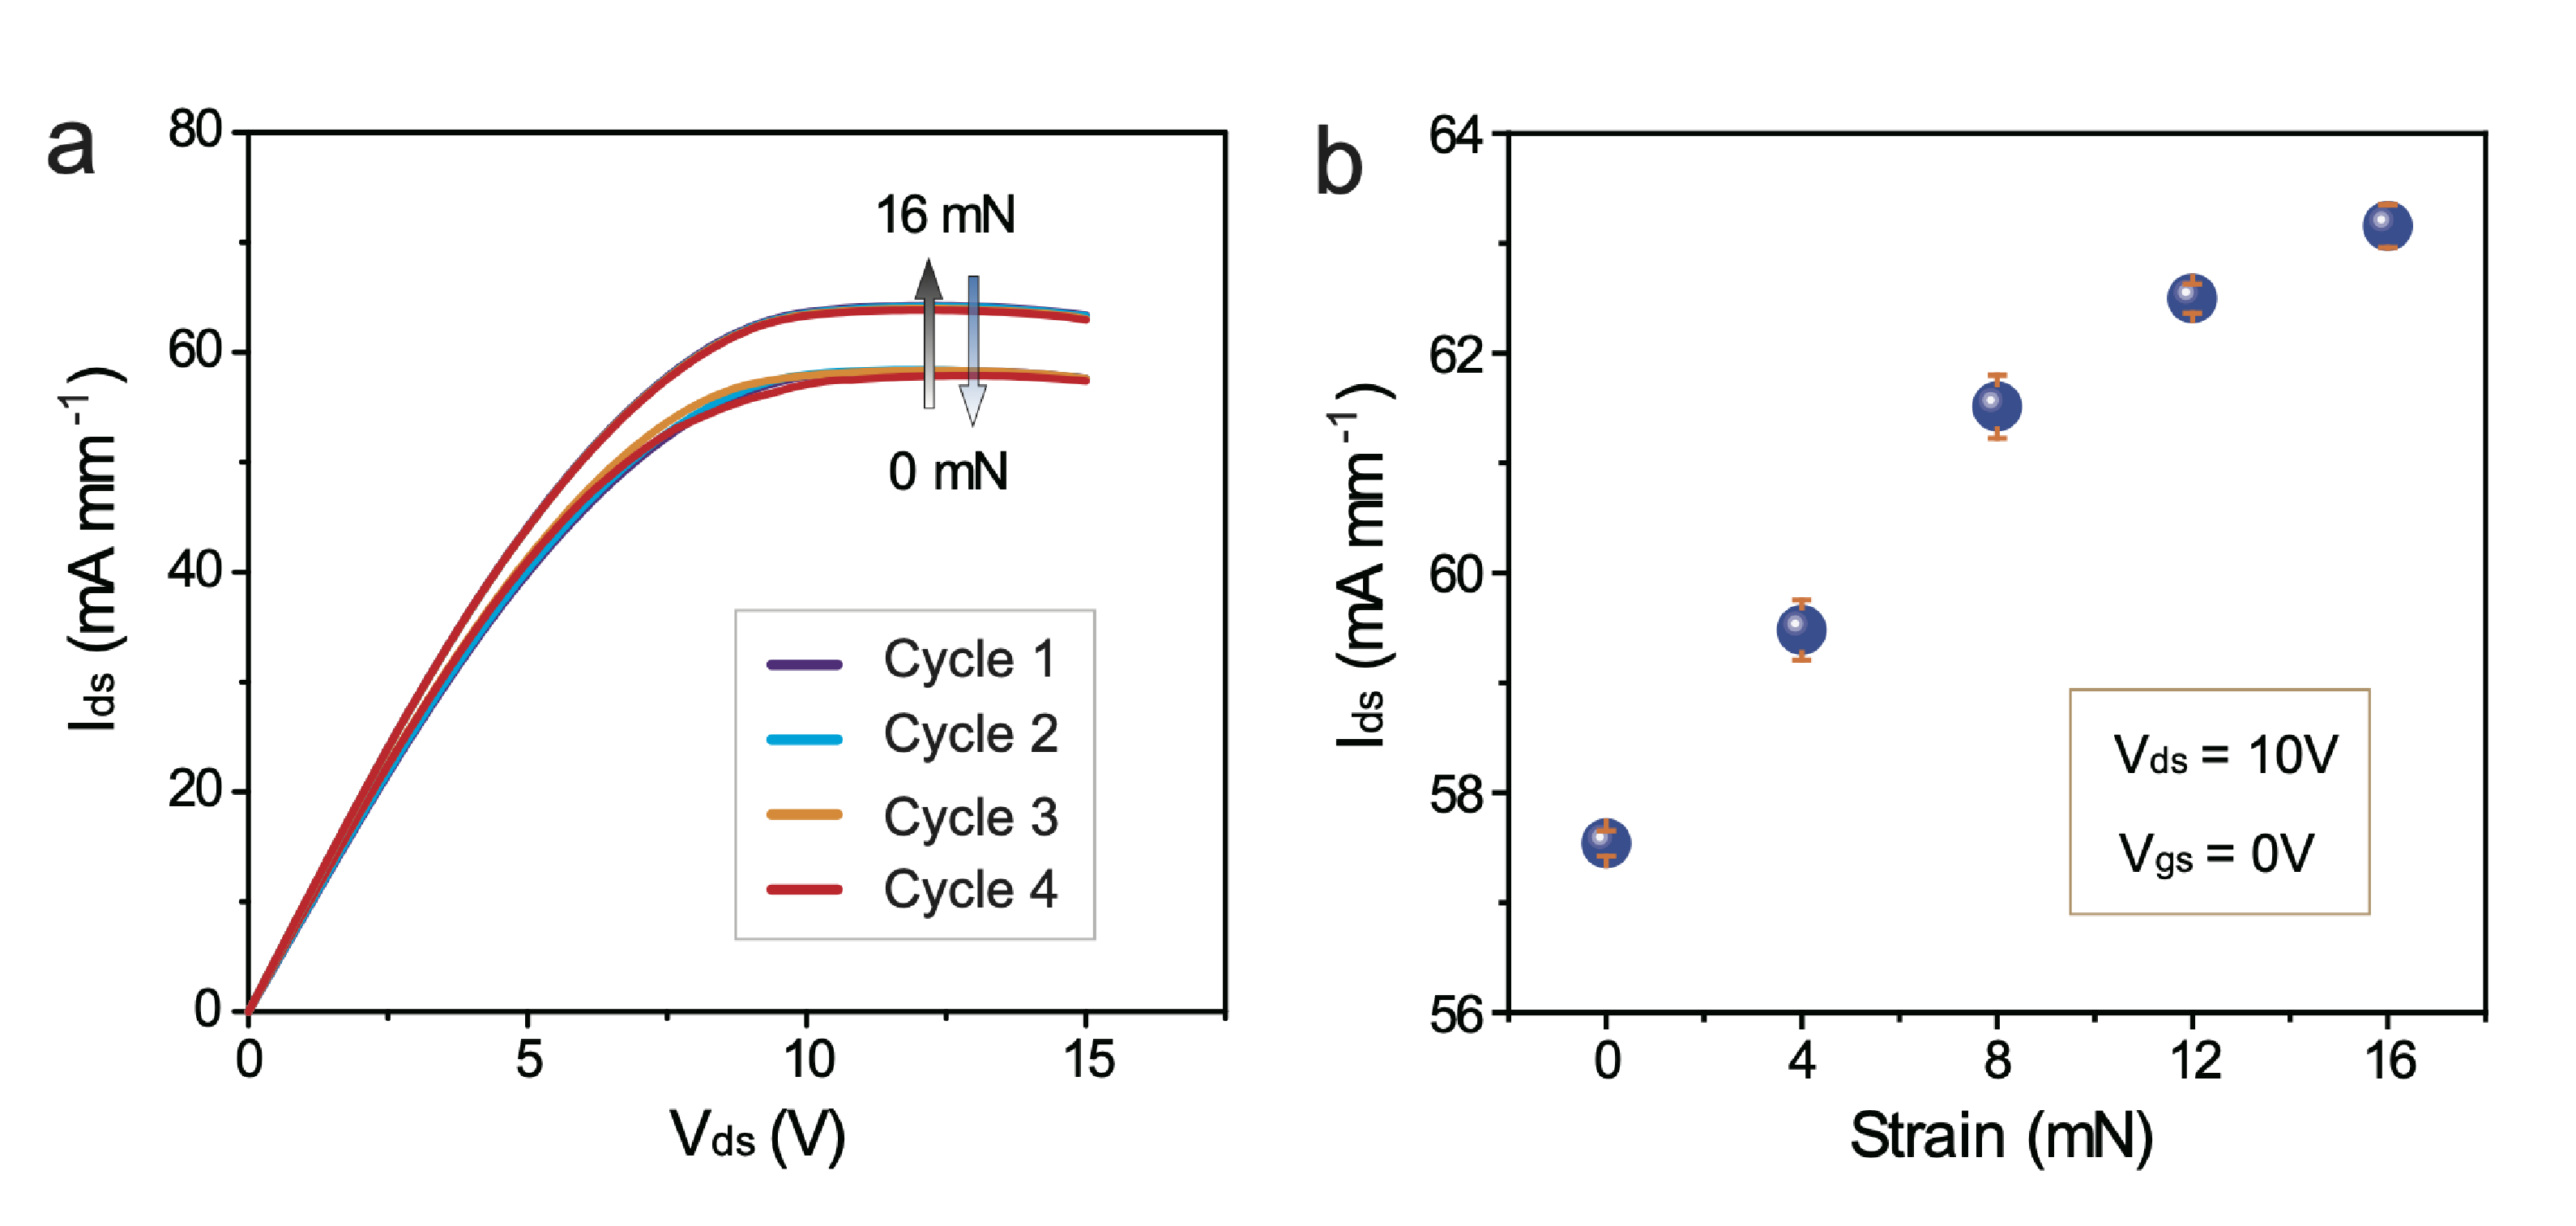
\includegraphics[width=0.9\textwidth]{ch3_modulation2}
\caption[Reproducible strain-dependent analysis of the SPD]{Reproducible strain-dependent analysis of the SPD. (a) Output characteristics in four consecutive cycles as the load and release of strain (0 /sim 16 \unit{mN}). (b) Statistical variation measured at $V_{ds}$ = \SI{10}{\volt}, $V_{gs}$ = \SI{0}{\volt} under external strain of 0 $\sim$ 16 \unit{mN}.}
\label{fig3:modulation2}
\end{figure}

\noindent changes). Moreover, the brain (gate) reserves the ultimate control over knee reflex. Besides, the reproducible procedures of loading or unloading multiple strains in response to the relative output power density of the SPD \index{Strain-controlled power MEMS devices (SPD)} are shown in \autoref{fig3:modulation1}c in cyclic tests, showing very good stable and repeatable performance for the strain-controlled devices.

\begin{figure}[H] 
\centering    

\includegraphics[width=0.9\textwidth]{ch3_repeat}
\caption[The reproducibility of the SPD under external strain]{The \index{Current!drain current} reproducibility under external strain. (a) Schematic illustration of the external strain program (load and release). Output characteristics to various strain of (b) 0 \unit{\mN}, (c) 4 \unit{\mN}, (d) 8 \unit{\mN}, (e) 12 \unit{\mN} and (f) 16 \unit{\mN} at $V_{ds}$=\SI{0}{\volt}, respectively.}
\label{fig3:repeat}
\end{figure}

To further investigate the reproducibility of the SPD \index{Strain-controlled power MEMS devices (SPD)} under external strain, the output currents can be obtained with the same batch sample after repeated loading/releasing strains (0, 4, 8, 12, and 16 \unit{\mN}) at a $V_{gs}$ of \SI{0}{\volt}. The strain-dependent output current \index{Output!current} curves and the statistical variation are shown in \autoref{fig3:modulation2}a, b, respectively. Highly stability and repeatability of the SPD \index{Strain-controlled power MEMS devices (SPD)} are clearly observed under each external strain (\autoref{fig3:repeat}). In addition, there is no obvious hysteresis in the strain response procedures, as shown in \autoref{fig3:modulation2}a. With the accretion of strain (0 $\sim$ 16 \unit{\mN}), the output current of the SPD shows a positive correlation (\autoref{fig3:modulation2}b). And the standard deviations under each strain (0, 4, 8, 12, and 16 \unit{\mN}) are calculated as 0.11$\%$, 0.27$\%$, 0.29$\%$, 0.13$\%$, 0.19$\%$, respectively. The SPD exhibits good reproducibility under \index{Current!drain current} the external strain stimuli, which is very suitable for strain-controlled power electronics.

\section{Working mechanism}
\label{sec:Working mechanism chapter3}

In this section we discuss the working mechanism \index{Physical!mechanism} of SPD, use the semi-classical physical model established in \autoref{ch:Theoretical Models of MEMS Cantilever Devices based on AlGaN/AlN/GaN Heterostructure} to demonstrate our experimental results and draw theoretical guidance for performance improvement. The analysis of the working principle of SPD is based on the piezotronics \index{Piezotronics} effect, that is, the coupling effect of the piezoelectric effect \index{Piezoelectric!effect} and the semiconductor properties existing in the III-V nitride AlGaN/AlN/GaN \index{AlGaN/AlN/GaN heterojunction} heterojunction. Because of the general piezoelectric polarization \index{Piezoelectric!polarization} and spontaneous \index{Spontaneous polarization} polarization effects in III-V nitrides, tensile and compressive strains of the lattice \index{Lattice!strain} will generate corresponding piezoelectric polarization charges \index{Piezoelectric!polarization charge} at the \index{Interface} interface, thereby changing the net polarization charge density at the \index{Interface} interface. In AlGaN/AlN/GaN heterojunctions, the change in the net polarization charge density at the interface affects the energy band of the heterojunction, which in turn affects a range of electrical properties. In the structural design of SPD, by introducing a cantilever \index{Cantilever} structure, we amplify the strain effect of external stress on the lattice, thereby amplifying the modulation \index{Modulation} characteristics of external stress on the output current \index{Output!current} and output power \index{Output!power} of \index{Strain-controlled power MEMS devices (SPD)} SPD, and successfully fabricated a MEMS device with strain-controlled power. The calculation results are shown in \autoref{tab:3.2} and \autoref{fig3:theory}, respectively.

\begin{table}[H]
\renewcommand\arraystretch{1.2}
\centering
\caption[The calculated result for $n_{2deg}$-strain relationship under the external force]{The calculated result for $n_{2deg}$-strain relationship under the external force}
\setlength{\tabcolsep}{7mm}{
\begin{tabular}{cc}
\hline \hline
Strain (\unit{mN}) & 2DEG Concentration ($\times 10^{13}$ \unit{\per\square\cm}) \\ \hline \hline
0           & 1.2099                          \\
4           & 1.3021                          \\
8           & 1.3431                          \\
12          & 1.3711                          \\
16          & 1.3918                           \\
 \hline \hline
\end{tabular}}
\label{tab:3.2}
\end{table}

The calculated conduction band \index{Conduction band} ($E_{c}$) of the AlGaN/AlN/GaN heterostructure is shown in \autoref{fig3:theory}a. And the enlarged $E_{c}$ of the AlGaN/AlN and AlN/GaN heterojunctions are shown in \autoref{fig3:theory}b, c, respectively. It is obvious that, as the increase of compressive strain on the \index{Cantilever} cantilever, the $E_{c}$ of AlGaN is lifted up while the $E_{c}$ of GaN is lowered down, which will deepen the potential well \index{Potential!well} of the AlN/GaN heterojunction. Owing to the reformation of $E_{c}$, the distribution of carrier concentration \index{Carrier!distribution} is calculated and, as a result, varies with external strains (\autoref{fig3:theory}d). It can be found that the peak value of carrier concentration \index{Carrier!concentration} increases with strain, indicating that more electrons are confined in the AlGaN/ AlN/GaN potential well. By virtue of the semiconductor physics theory, the 2DEG \index{Two-dimensional electron gas (2DEG)} sheet carrier concentration under various \index{Strain} strains is obtained by integrating the carrier concentration distribution along the c-axis. \autoref{fig3:theory}e shows that the 2DEG sheet carrier concentration has an increase with the loading strains ranging from 0 to 16 \unit{mN}, which contributes to the strain-responding output characteristics and power densities consequently. The calculated result for the relationships between 2DEG concentration and external force are listed in \autoref{tab:3.2}. The calculated 2DEG sheet carrier concentrations qualitatively match well with the experimental results (\autoref{fig3:repeat}b), where the $I_{ds}$ is proportional to the 2DEG \index{Two-dimensional electron gas (2DEG)} concentration.

\begin{figure}[H] 
\centering    
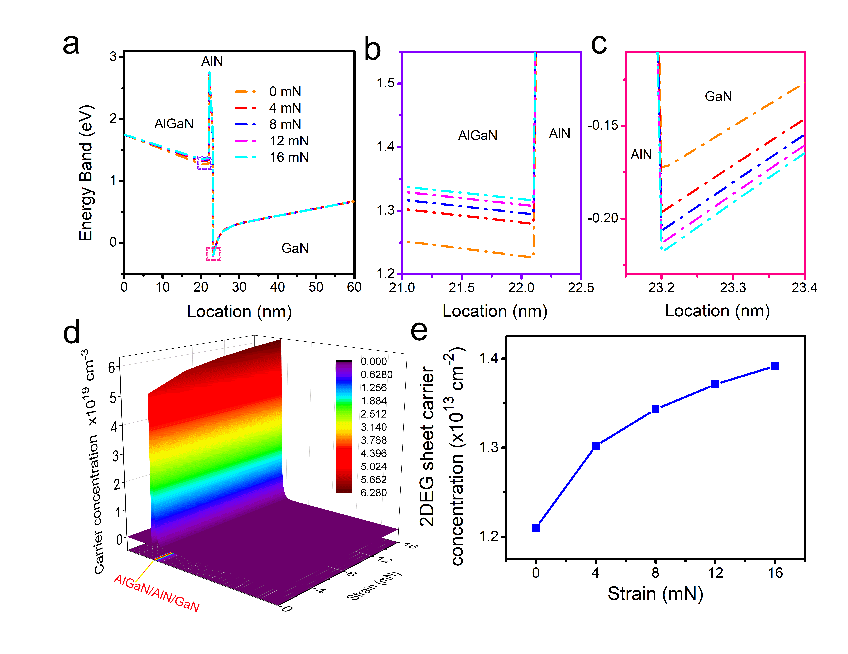
\includegraphics[width=0.9\textwidth]{ch3_theory}
\caption[The calculated energy band and 2DEG concentration in AlGaN/AlN/GaN heterojunction under external strains.]{The calculated energy band and 2DEG concentration in AlGaN/AlN/GaN heterojunction under external strains. (a) The conduction band under external strains. The enlarged conduction band of the AlGaN/AlN (b) and AlN/GaN (c). (d) The carrier concentration distribution and the 2DEG concentration (e) under external strains.}
\label{fig3:theory}
\end{figure}

\section{Summary}
\label{Summary}
In this chapter, we \index{Cantilever} present a bio-inspired strain-controlled power MEMS device based on the piezotronics effect which could directly control output power density with the mechanical stimuli. Ultra-high values of output power density ($\times 10^{13}$ \unit{\W\per\square\cm}) control under a weak force (\unit{mN}) control are achieved. The output power density of the SPD \index{Strain-controlled power MEMS devices (SPD)} increases to \num{2.72e3} \unit{\W\per\square\cm} under an external strain of 16 \unit{\mN}, which also exhibits a good sensitivity. The strain-induced piezoelectric polarization charge can contribute to modifying the conduction band \index{Conduction band} distribution at the local AlGaN/AlN/GaN heterojunction, and effectively adjust the concentration of 2DEG to tune/control the output current and power density of the SPD. In analogy to the ultimate control capability of the brain in the biological model, the gate voltage \index{Voltage!gate voltage} bias of the SPD can directly control the output power. This structure combines the advantages of high output power density and programmable gate-control response of AlGaN/AlN/GaN heterojunction HEMT by using the piezoelectric effect of flexible GaN-based \index{Cantilever} cantilevers. The SPD \index{Strain-controlled power MEMS devices (SPD)} will be very suitable for future AI applications including but not limited to autopilot, intelligent robots, and human-machine interface technologies.


\nomenclature{$V_{gs}$}{Gate voltage}
\nomenclature{$V_{ds}$}{Source-drain voltage}
\nomenclature{$I_{ds}$}{Source-drain current}
\nomenclature{$g_{m}$}{Transconductance}
\nomenclature{$F$}{External force}


\nomenclature[z-SPD]{SPD}{Strain-controlled power devices}

